
\chapter{PDR ベースの3次元屋内位置推定ライブラリの検討}
\thispagestyle{myheadings}
本章では,屋内位置推定ライブラリの要求仕様の検討およびその実装について述べる.
節3.1ではライブラリの要求仕様について詳述する.
節3.2では軌跡の画像と関数を用いて,どのような補正を行っているかを示す.
節3.3では気圧データを用いた3次元的な位置推定について示す.
% TODO: 2.PALKIAの名前を出してもいいかもしれない,本ライブラリの所を全てPALKIAで置き換える


\section{要求補正情報}
% TODO: 3.要求仕様ではなく要求補正情報の方がよさそう.要求仕様にするなら,柔軟性をもたせる設計にするとか書く必要がありそう.
% TODO: 3.要求仕様にしてこういう設計である必要があるという主張がいると思う.要求補正情報はおかしい
% TODO: これではまずい


PDRと他の情報を使ってライブラリを作成する上で,
どのような状況や環境が存在し補正に利用できるのかその具体的な例を考える必要がある.
例えば大学内や病院などのWi-FiのAPが多く設置されている場所では,
Wi-Fiの電波強度を利用した位置推定が有効である.
他の例として展示会場や大きなアトリウムなどの広い開放空間が考えられる.
このような場所ではWi-FiのAPの配置が難しく,
信号のカバレッジが不均一になりやすくWi-Fiを利用した位置推定は難しい.
このような場所の場合BLEビーコンを配置してその電波強度を利用した位置推定が有効である.
また2章で示したように\cite{pdr-wifi}\cite{pdr-ble}などのPDRと電波を利用した推定に関する研究は盛んに行われている.
このように電波を使った手法は多くの場所で有効であり,補正に利用可能な情報として重要度が高い.
そのため本ライブラリにおいても採用を行う.
他に補正に利用可能な情報としてフロアマップ情報がある.
フロアマップ情報は多くの場所で比較的入手が容易だと思われる.
そのため本ライブラリにおいても採用を行う.

磁気やカメラなどの情報は,磁気はデータが繊細であり電波と比べると補正に利用する難易度が高い,
カメラはプライバシーなどの問題があり本ライブラリの基礎段階においてこれらを採用しない.
また気圧センサは基礎段階として3次元空間を推定対象としないため採用しない.


\begin{figure}[ht]
	\centering
	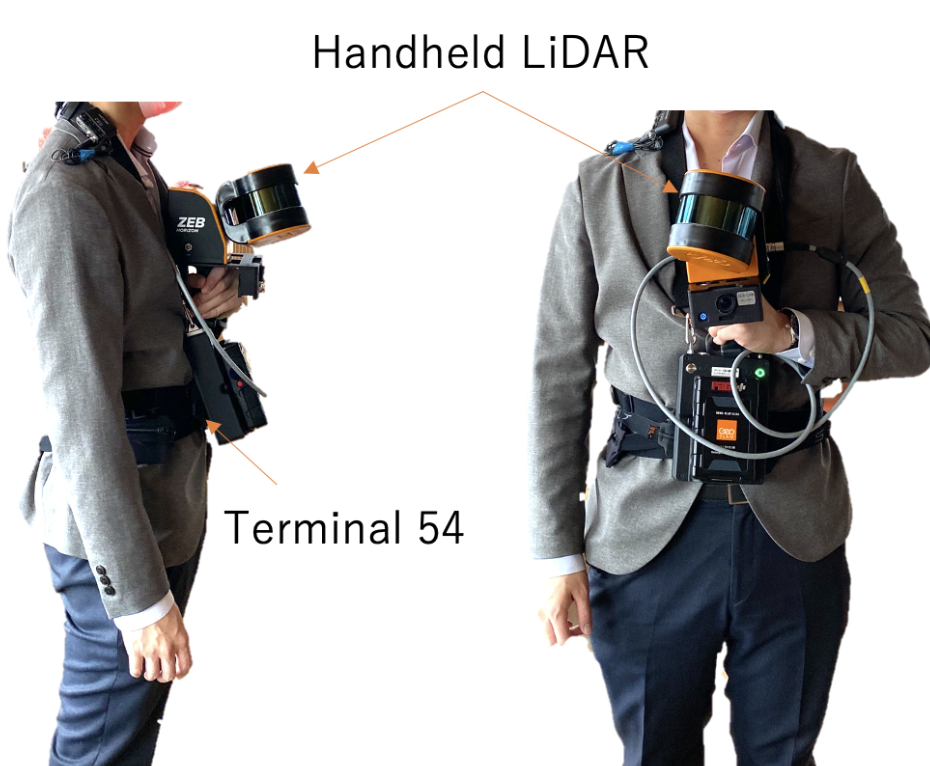
\includegraphics[width=\linewidth]{image/lidar.jpg}
	\caption{歩行者の装着器具}    \label{fig:step_detect}
\end{figure}







\section{xDR Challenge 2023環境における平面的な位置推定}

本ライブラリの補正アルゴリズム実装の検討および,その有効性の検証においてxDR Challenge 2023\cite{xdr}の環境を用いる.
xDR Challenge 2023 はPDRベンチマーク委員会が主催する屋内位置推定の精度を競うコンテストである.
このコンテストでは主催者が参加者に対して複数の訓練データを提供する.
被験者は腰にスマートフォンをつけた状態で,LiDARと呼ばれる距離測定技術を搭載したハンドヘルドLiDARを持ちBLEビーコンが配置された高速道路のサービスエリア内を歩く.
この過程で取得されたデータが訓練データとして提供される.
LiDARからは歩行者のフロアマップにおける歩行者の初期位置,終了位置,移動経路のデータが提供される.
LiDARは光を使って物体や壁までの距離を精密に測定できる技術であり,
このコンテストではLiDARから得られる提供データを正解軌跡として扱っている.
スマートフォンからは加速度,角速度,地磁気,各BLEビーコンのAP情報と受信電波強度が提供される.
フロアマップ情報,各ビーコンのフロアマップにおける基地局の位置情報は事前にコンテスト主催者側によって提供される.
そしてこの提供されたデータを基にコンテスト参加者は独自の推定アルゴリズムの開発を行い位置推定を行う.
本番で与えられるスコアを付けるためデータは訓練データと同様のフロアマップのデータが提供されるが,
LiDARからのデータは初期位置,初期姿勢,終了位置,終了姿勢のみが提供され,それ以外の情報を使って歩行者の移動軌跡を推定する.
xDR Challenge 2023の環境は,フロアマップ情報,各ビーコンの情報,スマートフォンからのセンサデータが提供されている.
そのためPDRと他の情報を使用した補正が可能であり,本ライブラリの要求仕様に適合している.
またライブラリを用いた処理の結果どのような補正の効果が得られるのかを検証する必要がある.
xDR Challenge 2023の環境は後述する評価システムが確立されており,本ライブラリの有効性を検証する環境が整備されている.
よってこの環境を基に補正アルゴリズム実装の検討および有効性の検証を行う.

\begin{figure}[ht]
	\centering
	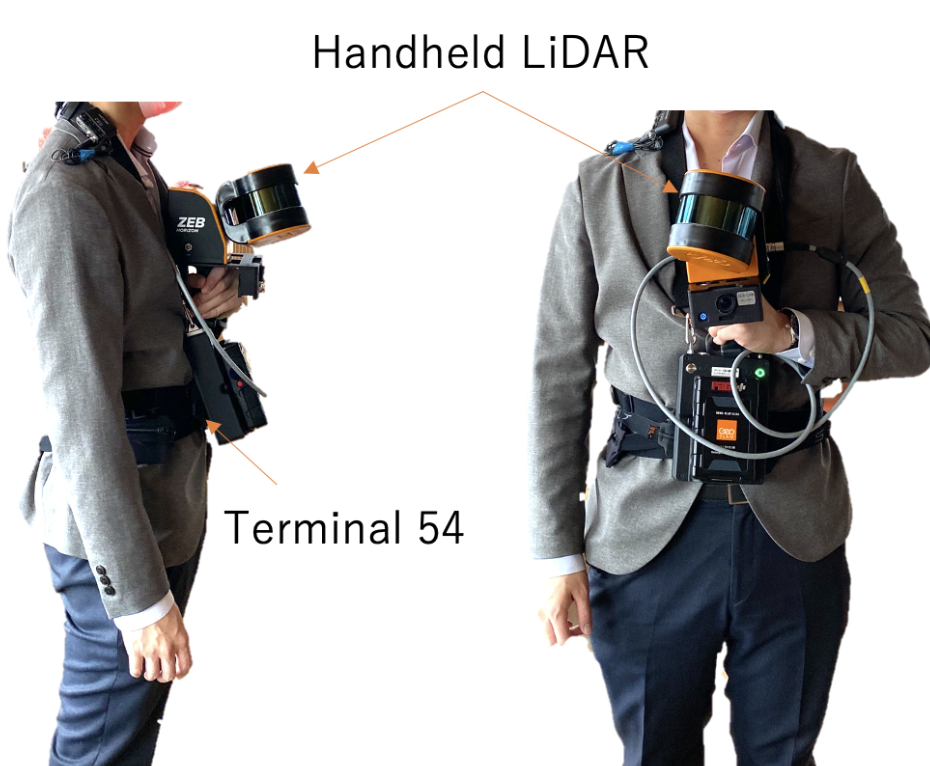
\includegraphics[width=\linewidth]{image/lidar.jpg}
	\caption{歩行者の装着器具}    \label{fig:step_detect}
\end{figure}



\subsection{基本的なPDR処理}

本ライブラリの基本的なPDR処理は,複数のクラスが協調して動作する設計となっている.
実装においては,コードの保守性と拡張性を重視し,Pythonの型ヒントやPandasライブラリを
効果的に活用している.特に,Pandasのデータフレーム構造を採用しており
大量のセンサデータに対する効率的な操作を実現している.また,時系列データのリサンプリングや
欠損値の補間,データの結合などの操作が容易に行えるため,センサデータの前処理や
解析に要する実装の複雑さを大幅に削減できる.
図\ref{fig:pdr-class}に示すように,PDREstimatorを中心として,StepEstimator,
OrientationEstimator,TrajectoryCalculatorの3つの主要なクラスが連携して
位置推定を行う.また,センサデータの管理はEnhancedSensorDataクラスが担当する.

\begin{figure}[H]
    \centering
    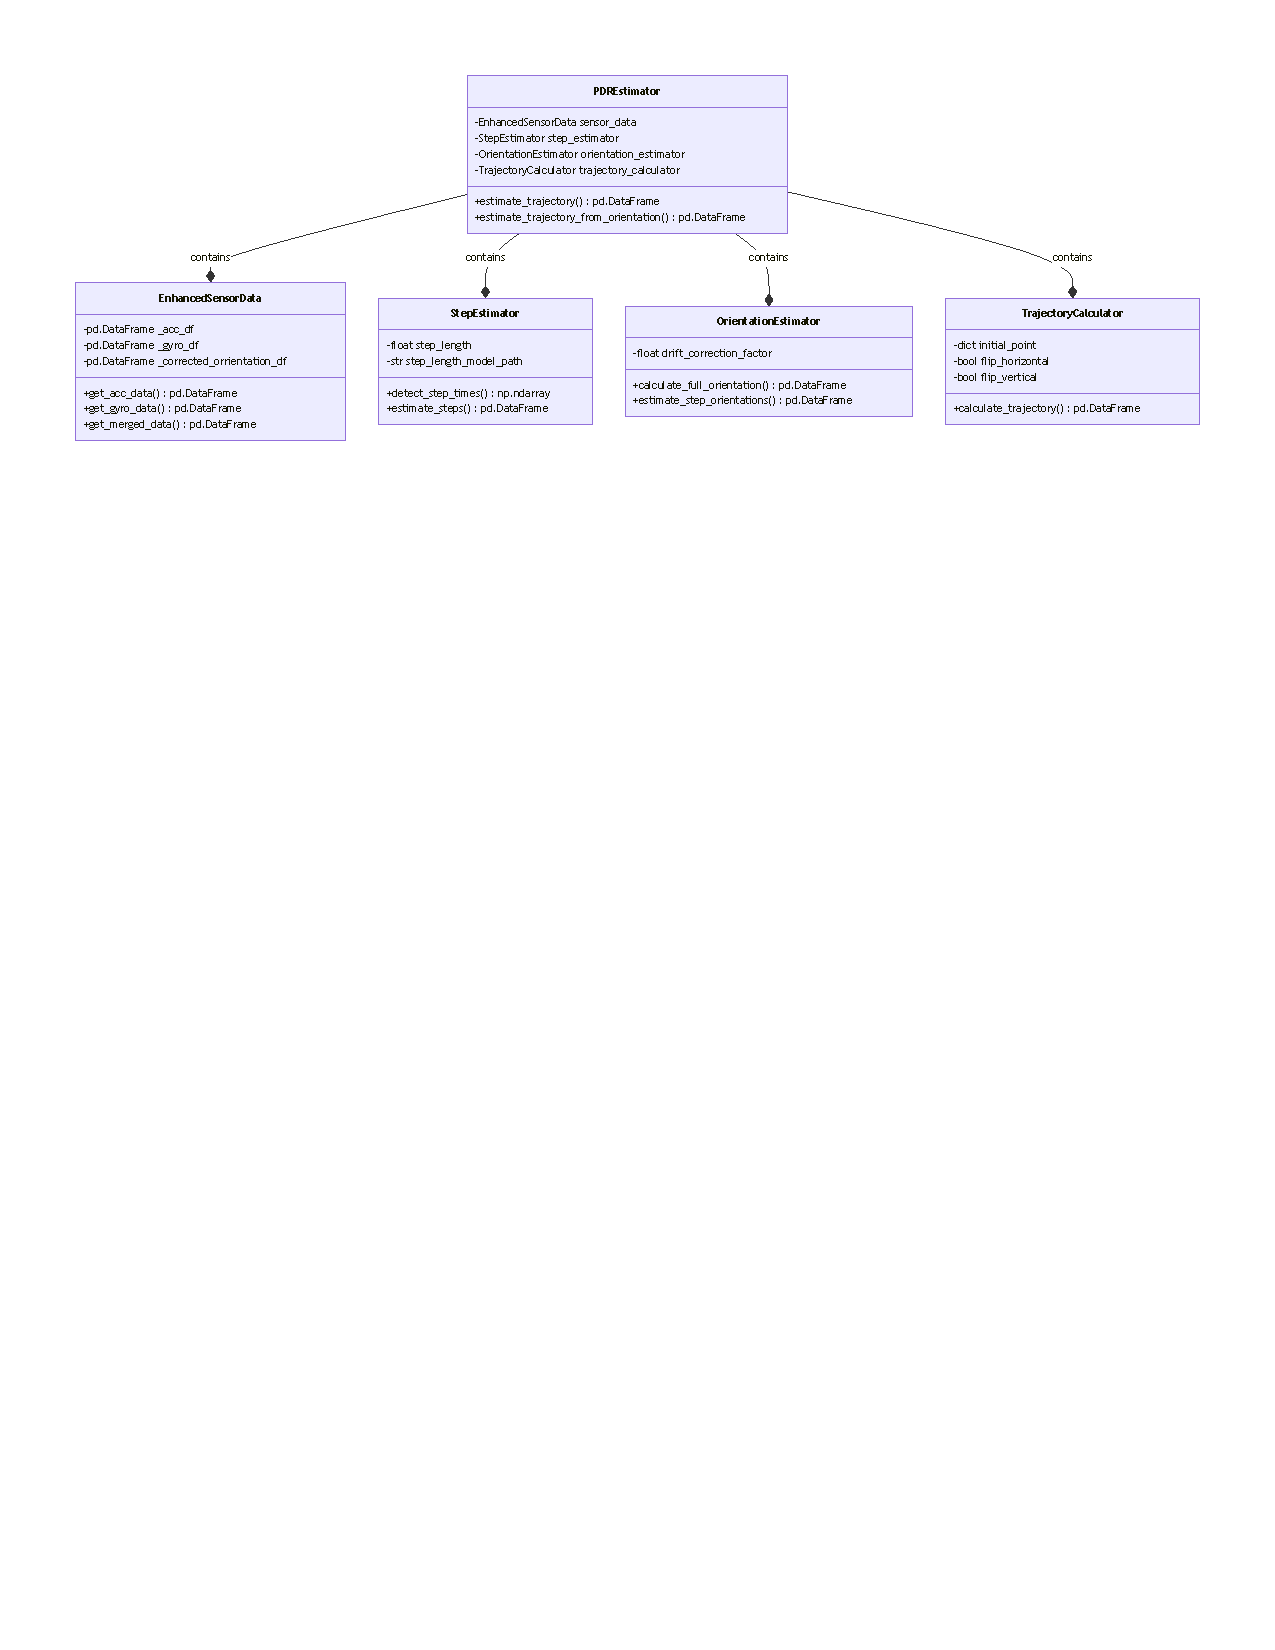
\includegraphics[width=\linewidth]{image/pdr-class-diagram.pdf}
    \caption{PDRの主要クラス構成}
    \label{fig:pdr-class}
\end{figure}

\subsubsection{システム構成}

本システムは,クラスベースの設計を行っている.各クラスの責任範囲を
明確に分離し,コードの理解性と保守性を向上させている.さらに,拡張可能な
インターフェース設計を採用しており,各クラスは明確なインターフェースを通じて相互に
連携するため,個々の実装の詳細を隠蔽しながら機能拡張が可能である.

各クラスの役割は以下の通りである:

\begin{description}
    \item[PDREstimator]\hfill 位置推定の中核となるクラスであり,他のコンポーネントを統括する.
    歩行検出,方向推定,軌跡計算の各処理を適切に連携させ,最終的な位置推定を行う.
    
    \item[EnhancedSensorData] 加速度,角速度などのセンサデータを管理する.データの前処理や
    同期処理を行い,他のコンポーネントに適切な形式でデータを提供する.
    
    \item[StepEstimator] 加速度データから歩行ステップを検出する.固定の歩幅を用いた
    シンプルな実装としており,拡張性を考慮した設計となっている.
    
    \item[OrientationEstimator] 角速度データから進行方向を推定する.ドリフト補正などの
    基本的な補正処理も行う.
    
    \item[TrajectoryCalculator] 検出された歩行ステップと推定された方向から,
    実際の移動軌跡を計算する.

\end{description}


\subsubsection{処理フロー}

PDRによる位置推定の処理フローを図\ref{fig:pdr-flow}に示す.本システムでは,センサデータの
入力から最終的な軌跡の出力まで,以下の段階を経て処理が行われる.

\begin{figure}[H]
    \centering
    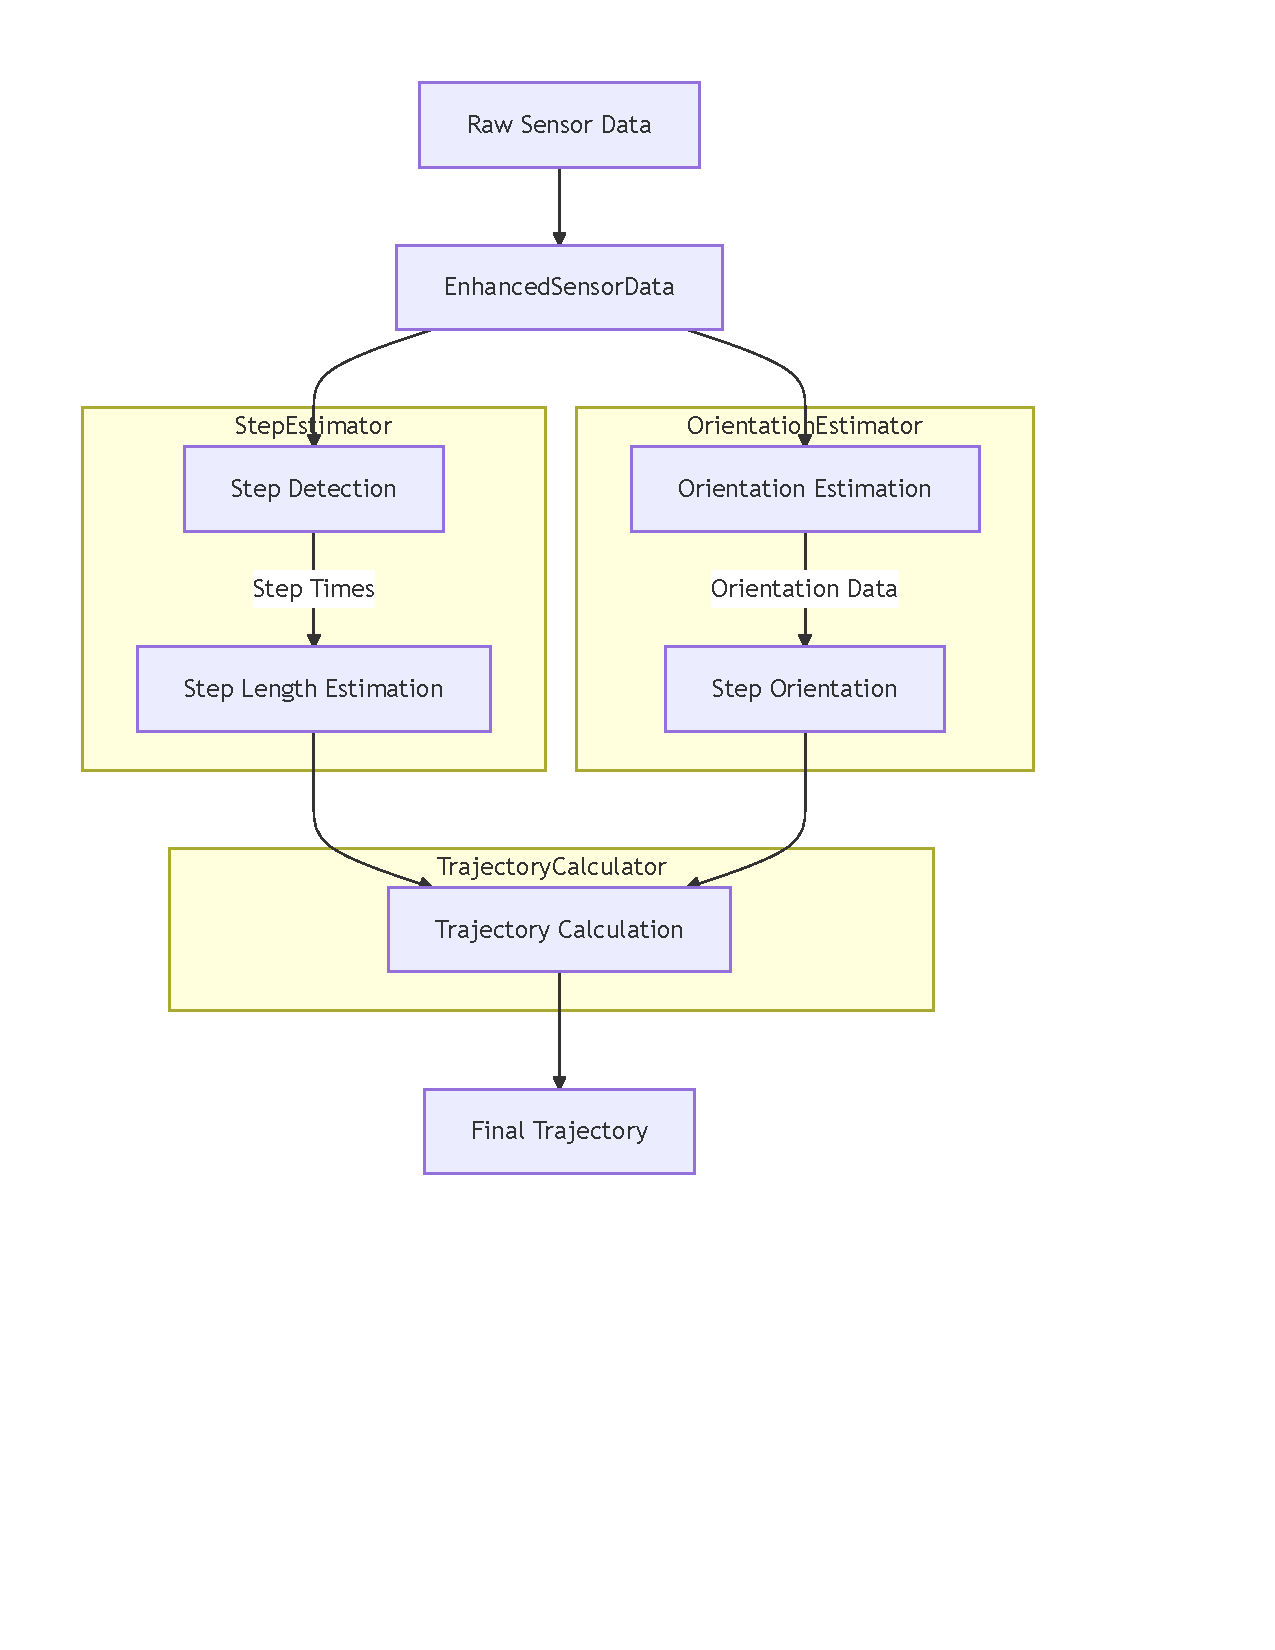
\includegraphics[width=\linewidth]{image/pdr-flow-diagram.pdf}
    \caption{PDRの処理フロー}
    \label{fig:pdr-flow}
\end{figure}

まずEnhancedSensorDataクラスにおいて,加速度センサと角速度センサから取得した生データの
前処理が行われる.前処理では,データの同期やノイズ除去などの基本的な処理に加え,
後続の処理で扱いやすい形式への変換が行われる.具体的には加速度データと角速度データの
サンプリング周波数の違いを考慮し,時系列データの補間処理を行い,両者のタイムスタンプを
一致させる.これにより後続の処理での時系列データの扱いが容易になる.


次に,StepEstimatorクラスにおいて歩行ステップの検出と歩幅の推定が行われる.
図\ref{fig:step_detect}に示すように,歩行ステップの検出では3軸加速度の
ノルムを計算し,その値が閾値を超えた時点を歩行ステップとして検出する.
具体的には,まず加速度のノルムに対して平滑化処理を適用し,
ノイズの影響を軽減する.
この際,単純な固定閾値ではなく,適応的な閾値処理を採用している.システムは
加速度信号の特性を継続的に監視し,平均値と標準偏差を用いて動的に閾値を
調整する.図\ref{fig:step_detect}の赤い破線で示されているように,
閾値は加速度の平均値に標準偏差の一定倍を加えた値として計算される.
この適応的な閾値の採用により,歩行速度の変化や個人差による加速度パターンの
違いに柔軟に対応できる.また信号の品質が時間とともに変化する
場合でも,安定した歩行検出が可能となる.図中の赤い点が,この適応的な
閾値処理によって検出された歩行ステップを示している.

同時にOrientationEstimatorクラスでは角速度データを用いた方向推定を行う.
図\ref{fig:step_timing}に示すように,角速度の積分により進行方向を算出する.
図中の青線は推定された進行方向の変化を,赤点は各歩行ステップでの方向を示している.
ただし積分処理には誤差の蓄積(ドリフト)という問題が存在する.
そのため本実装ではあらかじめドリフトの値が判明している場合,線形ドリフト補正を適用できるようにしている.
具体的には時間経過に比例する形でドリフト量を推定し,その影響を除去する処理を行う.

最後にTrajectoryCalculatorクラスにおいて,検出された歩行ステップと推定された
方向の情報を組み合わせて実際の移動軌跡を計算する.この過程では以下の式を用いて座標を逐次的に更新する:

\begin{equation}
x_{n+1} = x_n + L \cos(\theta_n)
\end{equation}
\begin{equation}
y_{n+1} = y_n + L \sin(\theta_n)
\end{equation}

ここで,$(x_n, y_n)$は$n$番目のステップでの位置,$L$は歩幅,$\theta_n$はその時点での
推定進行方向を表す.また,初期位置が与えられている場合は,その値を$(x_0, y_0)$として
使用する.さらに,座標系の定義に応じて,必要な座標変換(x軸やy軸の反転など)も
この段階で適用される.
% TODO: ここに中間報告で使用した計算が積み重なっていくのがわかる図があるといいかも

このように,各クラスが明確な役割分担の下で連携し,PDRによる位置推定を
実現している.また,この設計により,各処理段階での改良や機能追加が容易となっている.
例えば,より高度な歩行検出アルゴリズムの導入や,新たな方向推定手法の実装などが,
他のコンポーネントに影響を与えず可能である.


\begin{figure}[H]
	\centering
	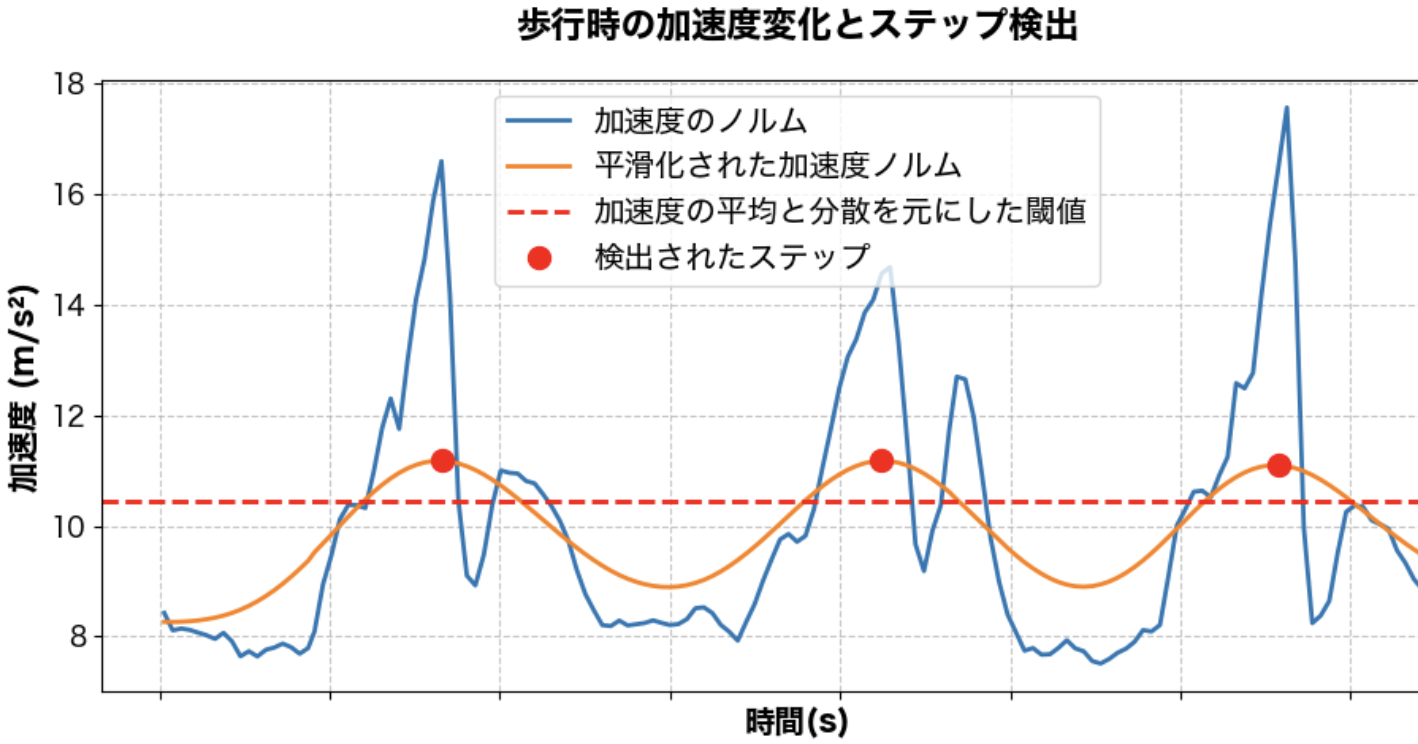
\includegraphics[width=\linewidth]{image/step_detect.jpg}
	\caption{加速度を利用したステップ検出}    \label{fig:step_detect}
\end{figure}


\begin{figure}[H]
	\centering
	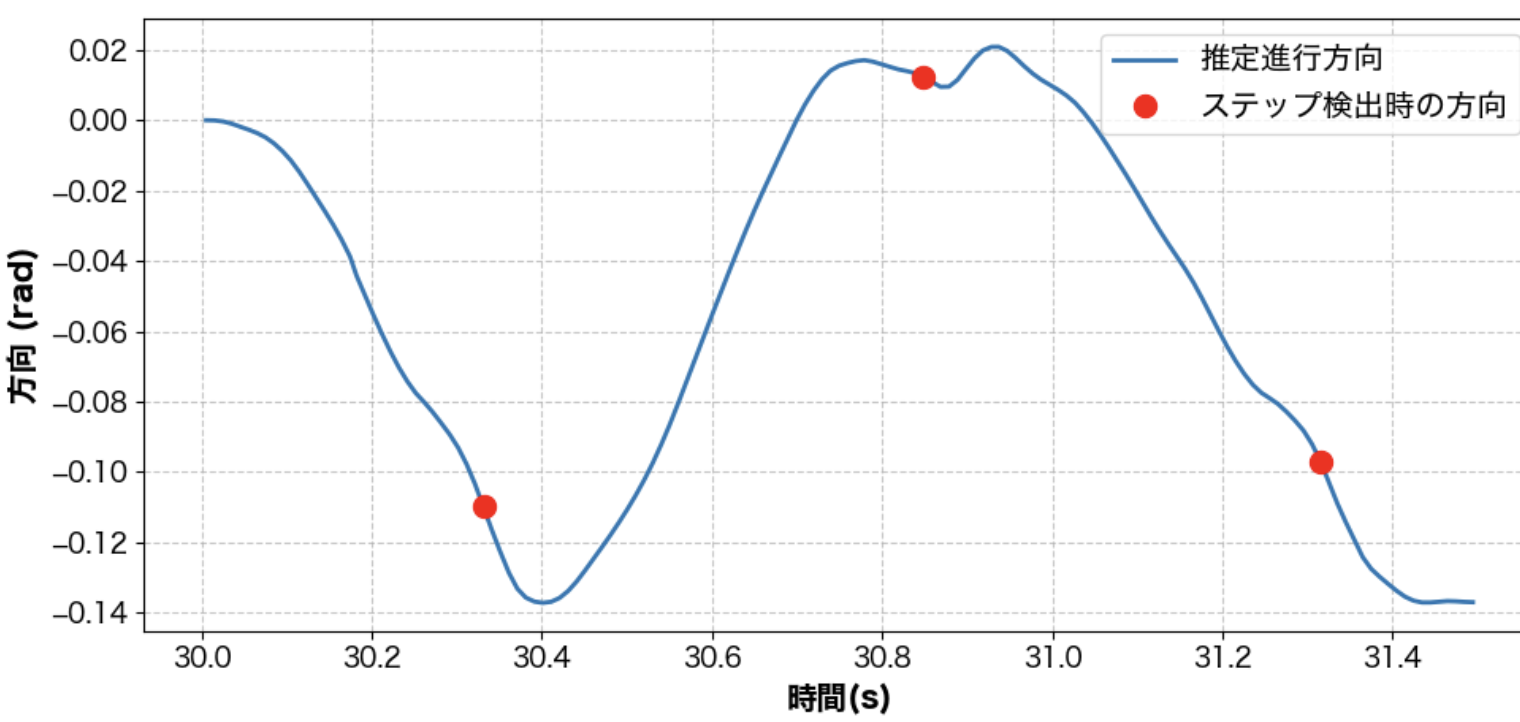
\includegraphics[width=\linewidth]{image/step_timing_angle.jpg}
	\caption{推定進行方向の変化}    \label{fig:step_timing}
\end{figure}


xDR Challenge 2023で与えられたトレーニングセンサーデータに対して処理を行った例を示す.
図\ref{fig:pdr}はPDREstimatorによる位置推定を行った結果である.
この図は2次元座標上に推定軌跡を表しており,軌跡の色は経過時間を表している.
紫色から赤色への変化が時間の経過を示している.
TrajectoryCalculatorに正解初期座標を与えた結果が図\ref{fig:pdr-move}である.
この図から分かるように,予め正解座標が判明している場合はPDRによる軌跡の初期位置を
適切に補正することができる.比較のため,LiDARで取得した座標を基に出力された
軌跡を図\ref{fig:gt-trajectory}に示す.これを本論では正解軌跡として扱う.
図\ref{fig:pdr-move}と図\ref*{fig:gt-trajectory}を比較すると,初期位置を補正した
PDRによる軌跡であっても,正解軌跡と比べて大きく異なっていることが分かる.
これはPDR特有の問題として,以下の2つの課題が存在するためである:

\begin{itemize}
    \item 相対的な移動の累積による軌跡の歪み
    \item 実世界の座標系における正確な位置の特定
\end{itemize}


続く3.2節では,これらの問題に対して軌跡補正クラスを用いたアプローチを示し,
PDRの軌跡を正解軌跡に近づけていく手法について詳しく説明する.


\begin{figure}[H]
    \centering
    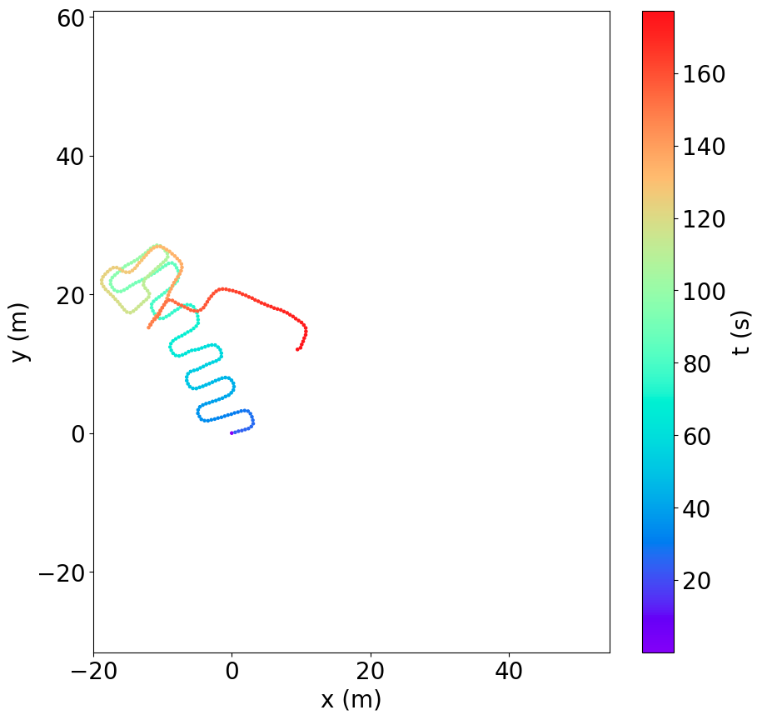
\includegraphics[width=\linewidth]{image/pdr.jpg}
    \caption{基本PDRの軌跡}    \label{fig:pdr}
\end{figure}


\begin{figure}[H]
    \centering
    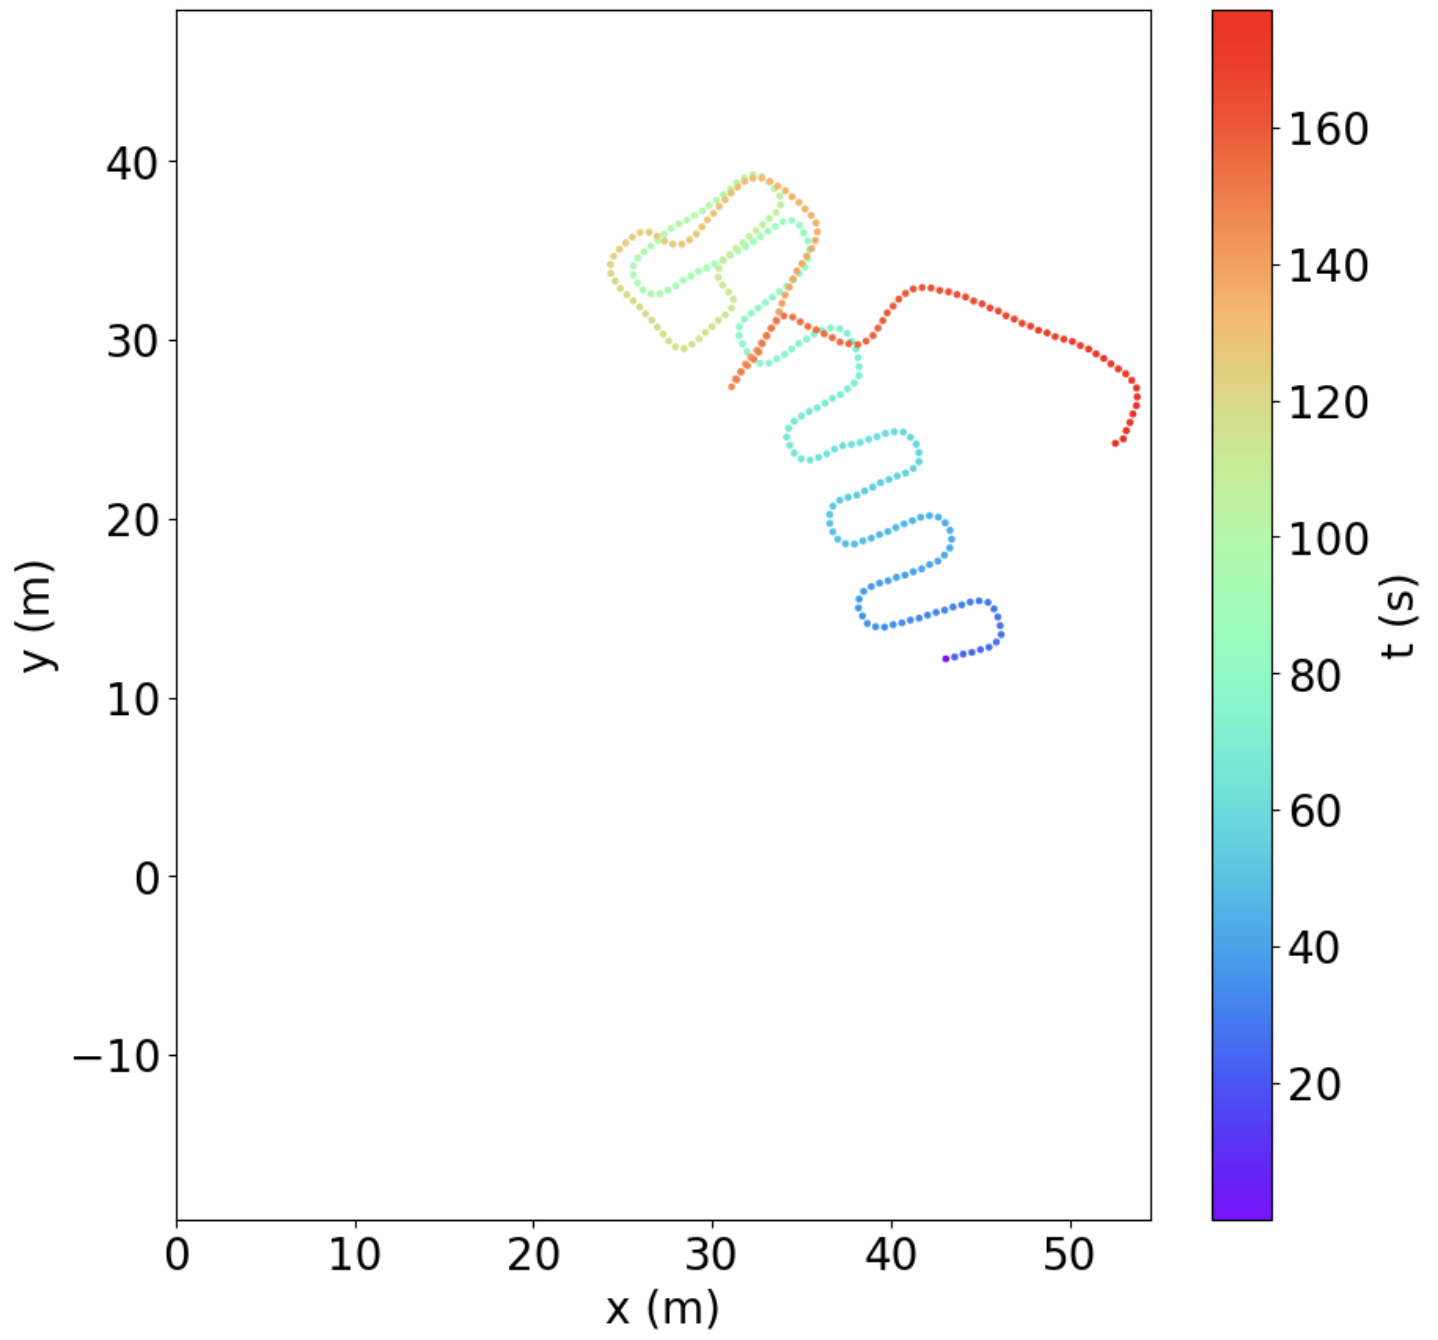
\includegraphics[width=\linewidth]{image/pdr-move.jpg}
    \caption{正解初期座標が存在}    \label{fig:pdr-move}
\end{figure}


\begin{figure}[H]
    \centering
    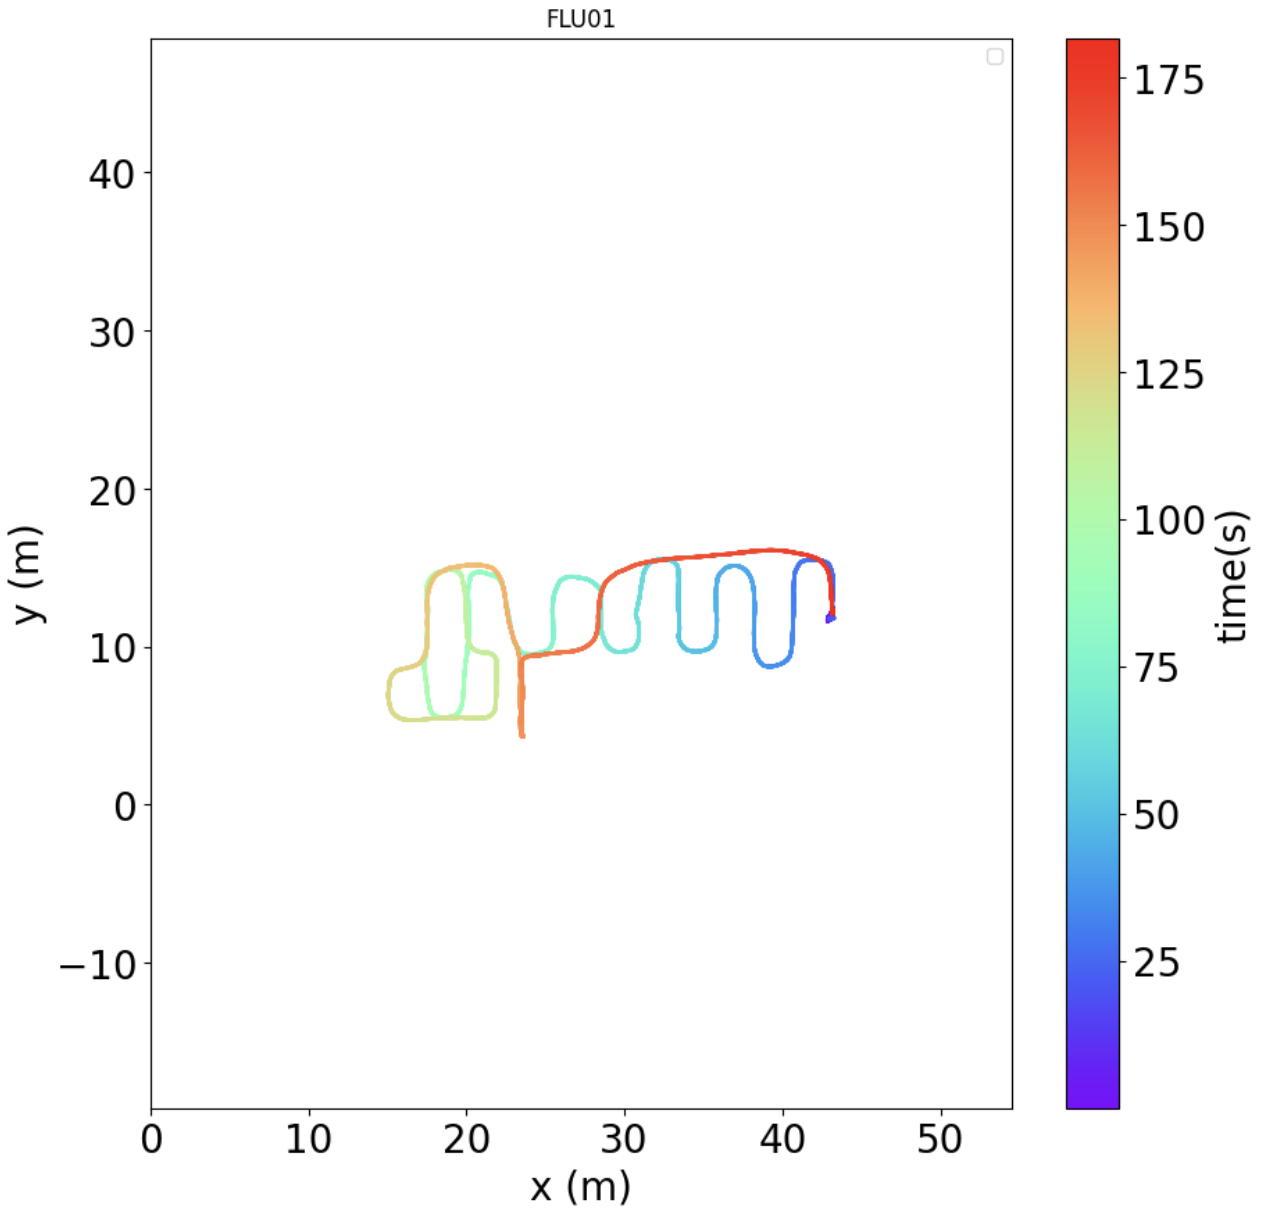
\includegraphics[width=\linewidth]{image/gt2.jpg}
    \caption{正解軌跡}    \label{fig:gt-trajectory}
\end{figure}














\subsection{軌跡の補正}

PDR処理で得られた軌跡には,前節で示したように2つの主要な課題がある.
これらの課題に対処するため,本ライブラリでは複数の補正手法を提供している.
各補正手法は異なるアプローチで軌跡の改善を試みるが,
これらを効果的に組み合わせることで,より高精度な位置推定が可能となる.


\subsubsection{補正手法の設計}

PDRによる位置推定の精度を向上させるため,本ライブラリは複数の補正手法を
組み合わせた設計を採用している.これらの補正手法を統合的に扱うために,
TrajectoryCorrectrorクラスを中心とした設計を提供している.
図\ref{fig:corrector-class}に示すように,補正処理はTrajectoryCorrector,
DriftCorrector,MapMatcher,WirelessSignalCorrectorの4つの主要なクラスから構成されており,
それぞれが特定の補正機能を担当している.各補正クラスは独立して実装されており,
TrajectoryCorrectorを介して緩やかに結合され,保守性と拡張性を実現している.

補正処理の柔軟な設定を可能にするため,TrajectoryCorrectorクラスは
Builderパターンを採用している.
これにより,複雑な補正処理の設直感的なインターフェースで提供が可能となっている.
利用者はwith\_floor\_map()やwith\_ble\_data()などのメソッドチェーンを使用して
利用可能な環境情報に応じて必要な補正手法を選択的に組み合わせられる.
Listing\ref{lst:trajectory-corrector}にその例を示す.
例のようにフロアマップのみが利用可能な環境では,MapMatcherによる補正のみを
指定し,BLEビーコンも利用可能な環境では両方の補正を組み合わせて使用する
できる.また各補正クラスは単体でも使用可能であり,特定の補正処理
のみを実行したい場合は,直接該当するクラスを利用を利用できる.

\begin{lstlisting}[caption={TrajectoryCorrectorの使用例},label=lst:trajectory-corrector,float=h]
# フロアマップのみを使用する場合
corrector = TrajectoryCorrector.builder(pdr_estimator)
    .with_floor_map(floor_map)
    .build()
# フロアマップとBLEビーコンを組み合わせる場合
corrector = TrajectoryCorrector.builder(pdr_estimator)
    .with_floor_map(floor_map)
    .with_ble_data(ble_scans, beacon_positions)
    .build()
\end{lstlisting}

この設計の特徴は,新たな補正手法の追加が容易である点にある.例えば,
磁気フィンガープリントを用いた補正手法を追加する場合,MagneticCorrector
クラスを新規作成し,TrajectoryCorrectorsBuilderに対応するメソッドを
追加するだけで良い.この際,既存の補正クラスのコードを変更する必要が
ないため,システムの安定性を保ちながら機能を拡張するできる.
また,各補正手法は独立して実装されているため,個々の手法の改良や
バグ修正も他の機能に影響を与えず実装できる.

図\ref{fig:corrector-sequence}は,これらの補正処理の連携を示している.
TrajectoryCorrectorsBuilderを通じて必要な補正手法を指定し,buildメソッド
によってTrajectoryCorrectorのインスタンスを生成する.その後,
estimate\_and\_correct\_trajectoryメソッドを呼び出すと,指定された
補正手法が順次適用され,最終的な補正軌跡が得られる.この処理フローにより,
複数の補正手法を組み合わせた高度な位置推定が可能となっている.

\begin{figure}[H]
    \centering
    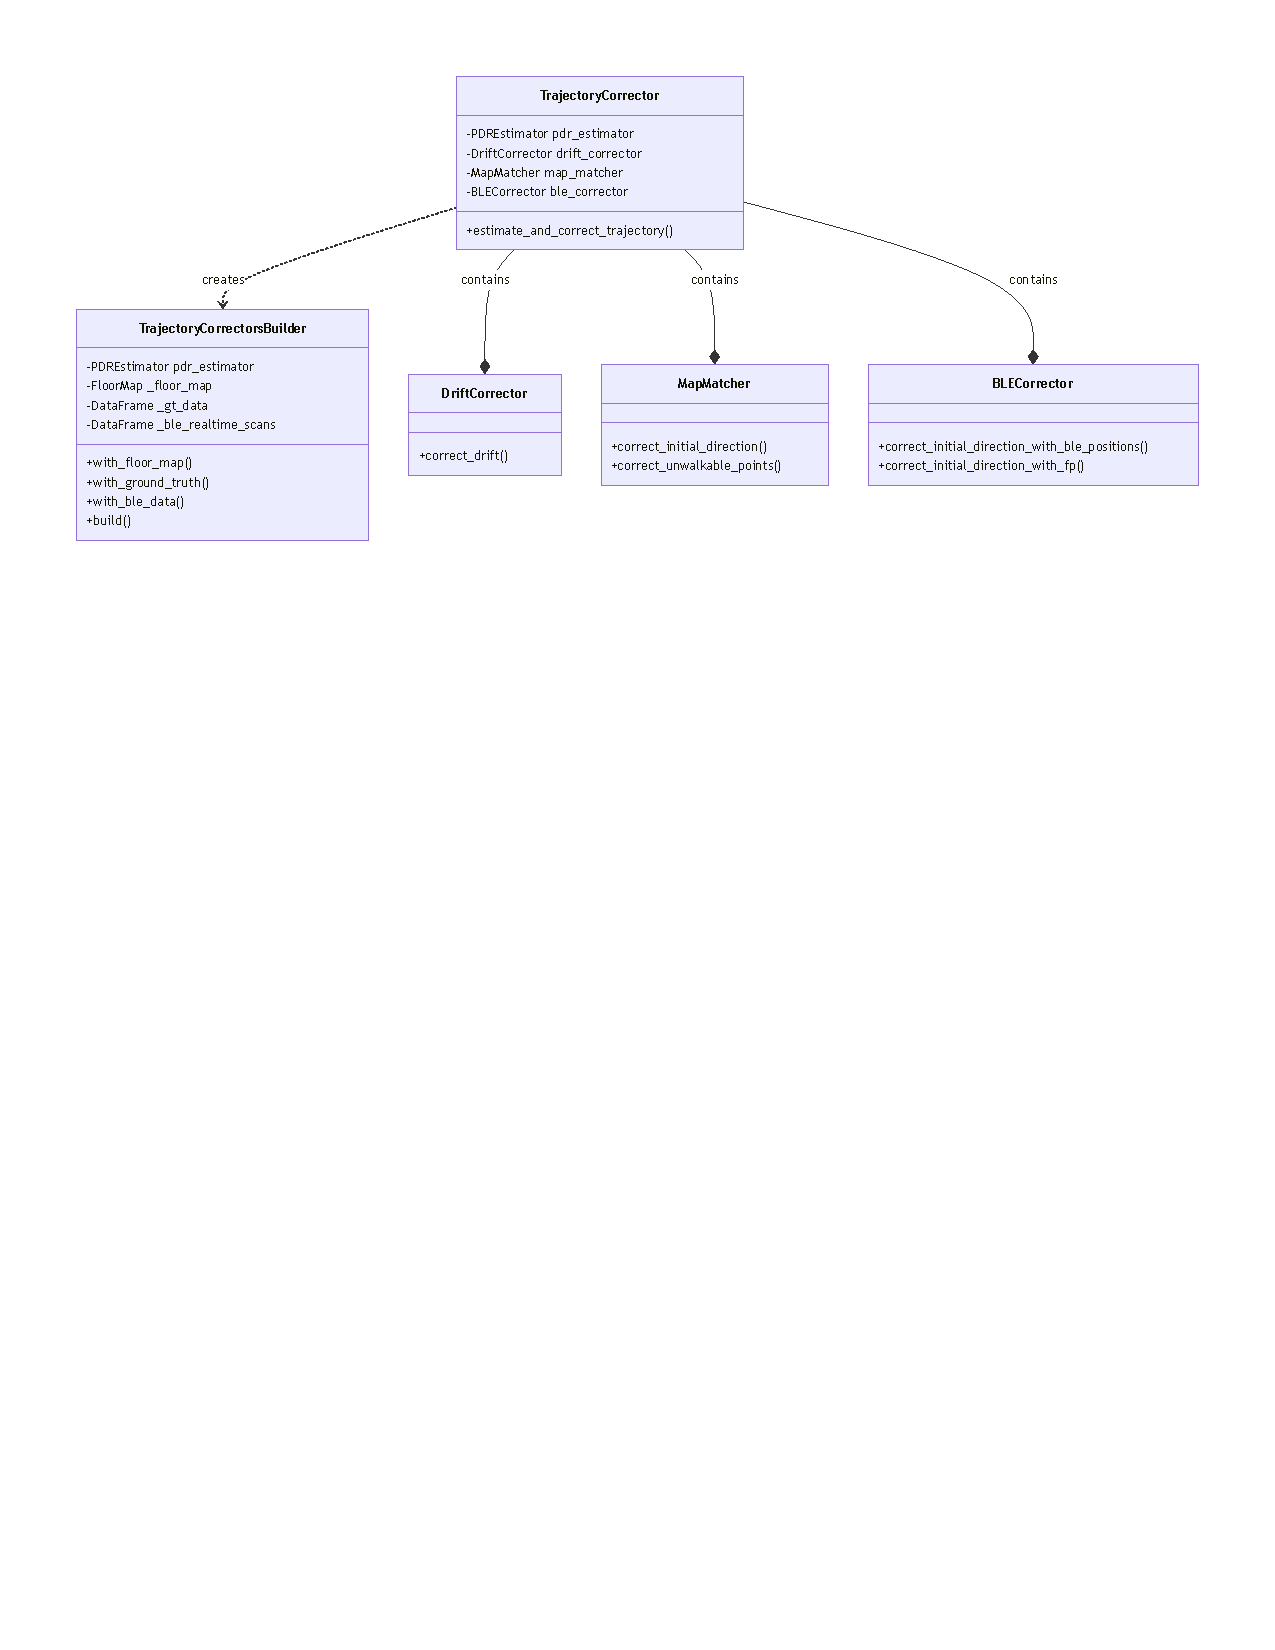
\includegraphics[width=\linewidth]{image/corrector-class-diagram.pdf}
    \caption{補正における主要クラス設計}
    \label{fig:corrector-class}
\end{figure}
% TODO:3.図の文字が小さくて読めない,図を大きくするといいかも

\begin{figure}[H]
    \centering
    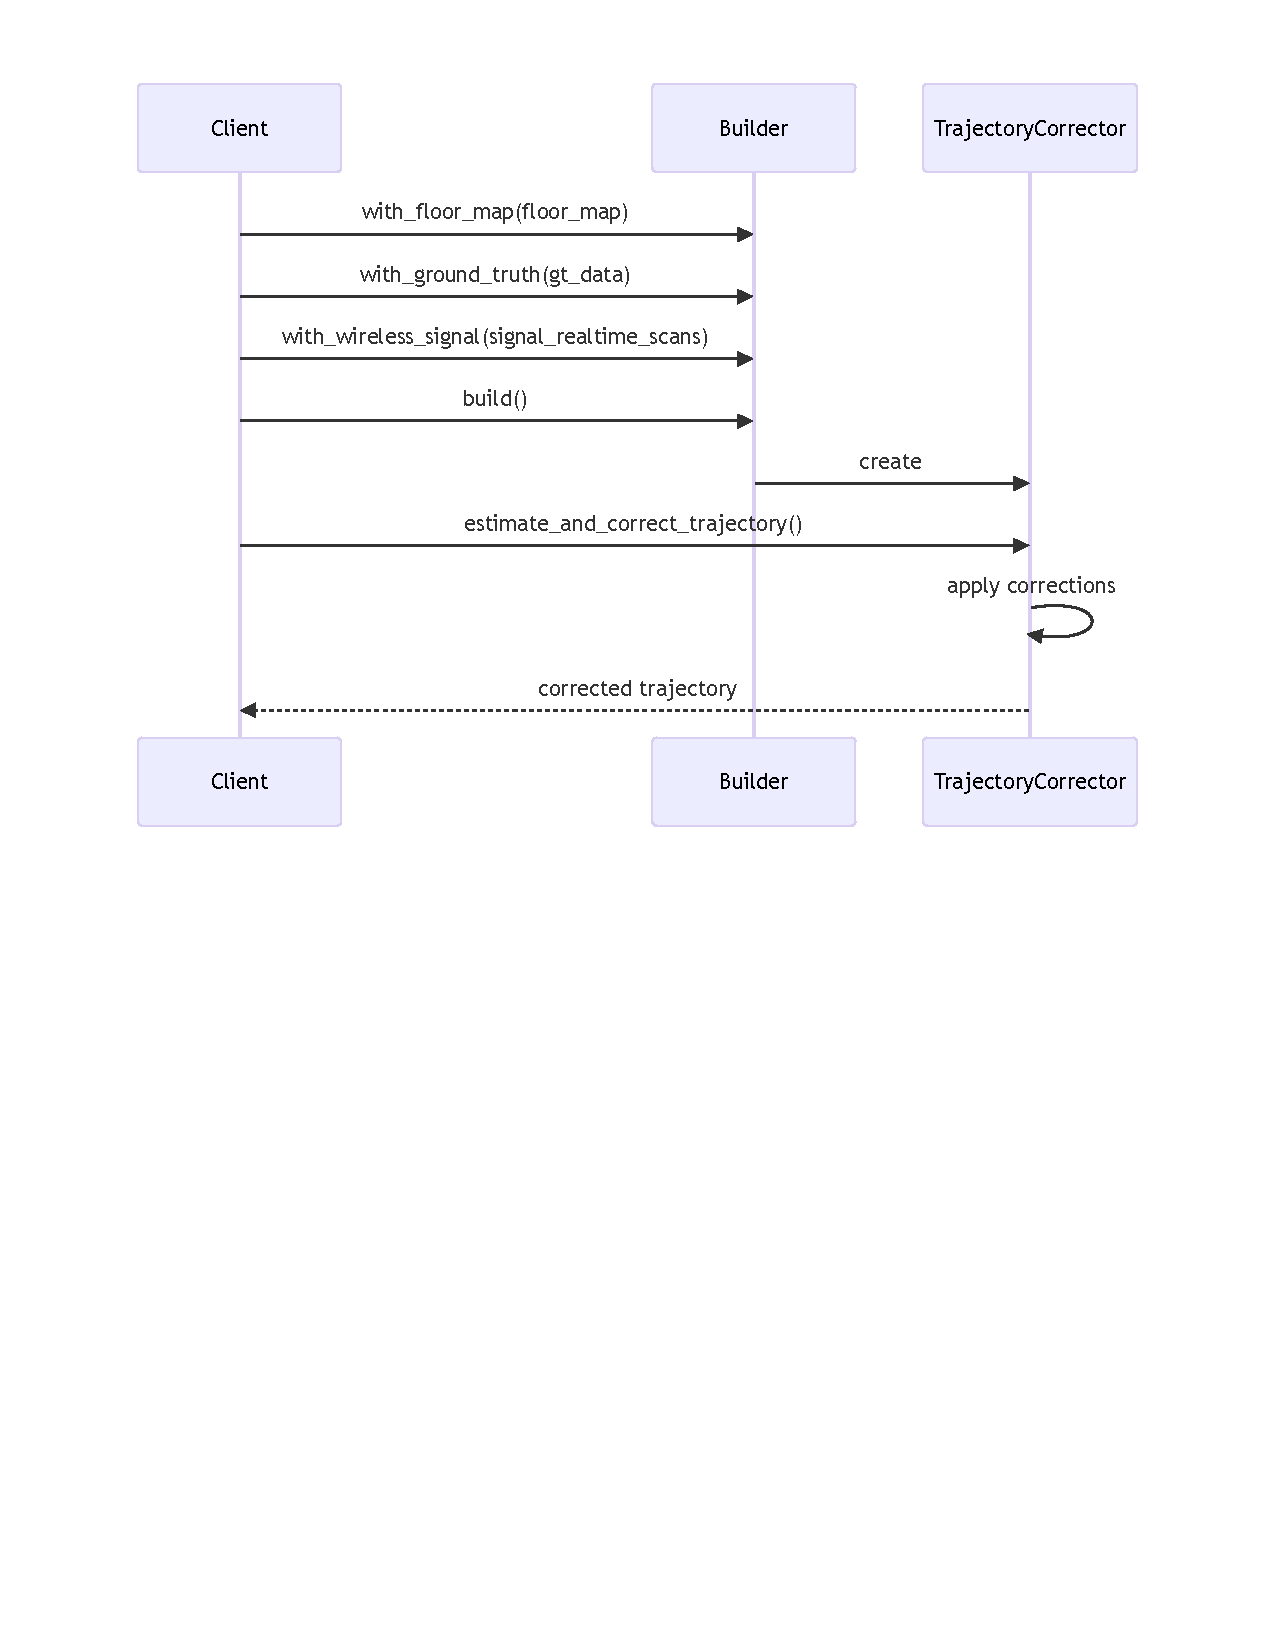
\includegraphics[width=\linewidth]{image/corrector-flow-diagram.pdf}
    \caption{補正の処理フロー}
    \label{fig:corrector-sequence}
\end{figure}

\subsubsection{既知の座標を使用したドリフトの除去}

図\ref{fig:pdr-move}の軌跡にはPDR特有のドリフト現象が見られる.
PDRでは角速度から進行方向を求めてその方向を元に歩行軌跡を描くため,
角速度センサーにわずかでも誤差が含まれると,時間経過とともにその誤差が
累積し,軌跡の形状が本来の軌跡から大きく外れていく.この問題に対処するため,
本ライブラリではDriftCorrectorクラスを提供している.

この手法を利用するために必要な情報は既知の座標データである.既知の座標データには
特定の時刻における歩行者の位置情報が含まれている.このデータは
任意の時刻の座標である必要はなく,軌跡の始点や終点など,いくつかの
時点での位置情報があれば補正が可能である.また,補正の精度は
与えられる既知の座標の数や,座標間の時間間隔によって変化する.
この手法の利用例をlisting \ref{lst:drift-corrector}に示す


% TODO 2.captionの名前は検討した方がいいかも
% TODO 2.やっぱり関数ものせた方がいいかも,何の情報を入力するという部分は必要かもしれない(要検討)
% TODO: 2.しかし軌跡を引数に与えていないから違和感がある.内部的にはenhanceSensorDataの角度をみて修正してる.コードごと消すか
\begin{lstlisting}[caption={DriftCorrector},label=lst:drift-corrector,float=h]
# 正解座標データ
ground_truth = pd.DataFrame({
    'ts': [0, 180],           # タイムスタンプ(秒)
    'x': [15.0, 15.0],       # x座標(メートル)
    'y': [19.0, 19.0]        # y座標(メートル)
})

# DriftCorrectorの初期化と補正の実行
drift_corrector = DriftCorrector(
    pdr_estimator=estimator,  # PDREstimatorインスタンス
    gt_data=ground_truth      # 正解座標データ
)
\end{lstlisting}



DriftCorrectorクラスは,正解座標との比較に基づいて角速度データの累積誤差を
補正する.この補正処理は以下の式で表される:

\begin{equation}
    \theta'(t) = \theta(t) - (d \times t)
\end{equation}

ここで,$\theta'(t)$は時間$t$における補正後の角度,$\theta(t)$は
補正前の角度,$d$はドリフトの大きさを表す.この式は時間経過に伴う
ドリフトの累積効果を線形モデルで近似し,補正を行う.
最適なドリフト値$d$の決定には,既知の座標との誤差を最小化するアプローチを
採用している.具体的には,補正後の軌跡の終点と既知の座標との
ユークリッド距離$E$を以下の式で計算する:

\begin{equation}
    E = \sqrt{(x_{n+1} - x_n)^2 + (y_{n+1} - y_n)^2}
\end{equation}

ここで,$(x_n, y_n)$は既知の座標,$(x_{n+1}, y_{n+1})$は補正された
軌跡の終点を表す.DriftCorrectorはこの距離$E$が最小となるドリフト値をグリッドサーチにより探索する.
探索範囲はデフォルトで[-0.02, 0.02] rad/sとしている.この範囲は一般的なMEMSジャイロセンサーの
バイアス誤差の特性を考慮して設定されている.より大きな範囲を設定すると,
センサーの誤差だけでなく,実際の方向転換まで補正してしまう可能性がある.
また,この値の範囲は外部から変更可能であり,使用するセンサーの特性に応じて調整できる.

% TODO:2.ここにパワポにあるようなグリードサーチしている感がある図を載せるといいかも

図\ref{fig:pdr-remove-drift}に示すように,ドリフト補正後の軌跡は
元の軌跡と比較して正解軌跡の形状に近づいている.特に,既知の座標間の
距離が近い場合に効果的である.また,2点以上の既知の座標が存在する場合も,
同様のアプローチで補正を行うことが可能である.

\begin{figure}[H]
	\centering
	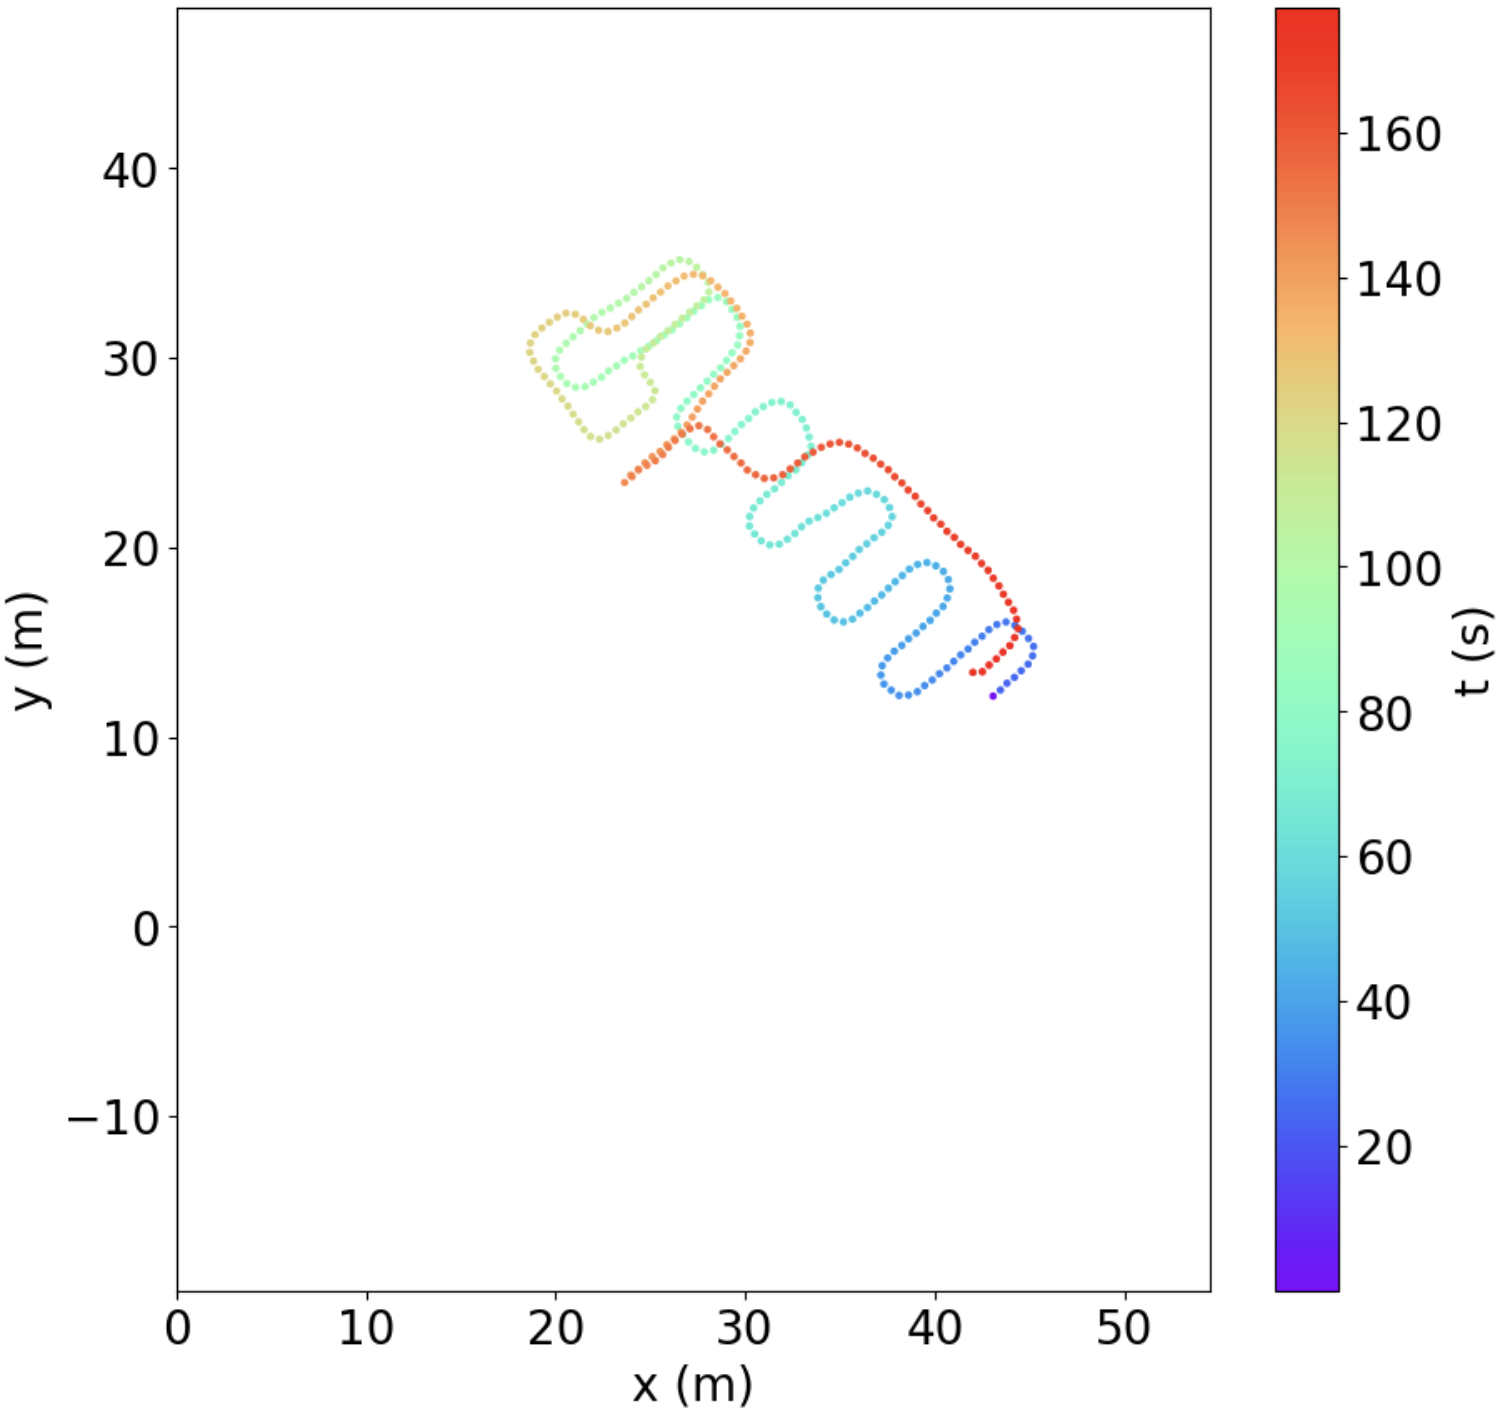
\includegraphics[width=\linewidth]{image/pdr-remove-drift-two.jpg}
	\caption{ドリフト補正後の軌跡}    \label{fig:pdr-remove-drift}
\end{figure}




\subsubsection{フロアマップを用いた初期進行方向の補正}

図\ref{fig:pdr-remove-drift}の軌跡には,初期進行方向の誤差という重要な
問題が残されている.初期進行方向が誤っていると,その後の全ての推定位置が
実際の移動経路から大きく逸れることになる.この問題に対処するため,本ライブラリ
ではMapMatcherクラスを提供している.

この手法を利用するために必要な情報はフロアマップ情報である.フロアマップは
建物の構造を表す2次元の画像データとして与えられ,歩行可能な領域と
歩行不可能な領域を区別できる必要がある.図\ref{fig:floor-map}に実際の
フロアマップを示す.このマップでは灰色の部分が歩行可能領域,白色の部分が
歩行不可能領域を表している.
この手法の利用例を\ref{lst:rotate-trajectory-using-ble-fingerprint}に示す


% TODO: 2.修正関数の呼出しの部分は削除したがそれでよかったのだろうか
% TODO: 2.captionの名前は検討した方がいいかも
\begin{lstlisting}[caption={MapMatcherの使用例},label=lst:rotate-trajectory-using-ble-fingerprint,float=ht]
# フロアマップの読み込み
floor_map = FloorMap(
    floor_name="floor_5",
    floor_map_path="floor_5.png",  # 二値化された画像
    dx=0.01,  # x方向の1ピクセルあたりの距離(m)
    dy=0.01   # y方向の1ピクセルあたりの距離(m)
)

# MapMatcherの初期化
map_matcher = MapMatcher(
    pdr_estimator=estimator,
    floor_map=floor_map
)
\end{lstlisting}

% TODO 3.どのような情報をあたえるのが重要かという所を強調したい.今回の場合はフロアマップの情報を与えるのが重要
MapMatcherクラスは,フロアマップの構造的特徴を利用して最適な初期進行方向を
推定する.この手法は,多くの屋内環境において壁や通路が直交する形で構成されているという特徴を活用している.
図\ref{fig:floor-map}に実際のフロアマップを示す.
このマップの灰色の部分が歩行可能領域であり,白色の部分が歩行不可能領域である.
図\ref{fig:floor-map}に示すような実際のフロアマップでは,
歩行可能な経路の多くが建物の主軸に沿って配置されている.

\begin{figure}[H]
	\centering
	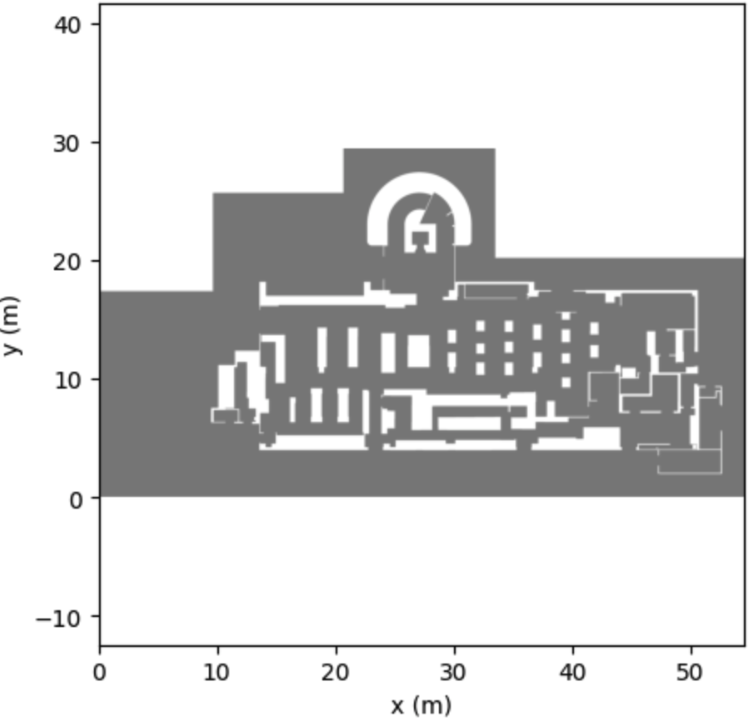
\includegraphics[width=\linewidth]{image/floor-map.jpg}
  \caption{フロアマップ情報} \label{fig:floor-map}
\end{figure}

初期進行方向の推定は,以下の2段階のプロセスで行われる:

第一段階では,軌跡のx軸,y軸に対して平行な成分の割合を最大化する角度を探索する.
具体的には,進行方向の角度が垂直方向(90度または270度)に対して±0.1ラジアン以内,
または水平方向(0度または180度)に対して±0.1ラジアン以内の歩行ステップを平行な
成分としてカウントする.この閾値は,人間の通常の歩行では廊下や通路に対して
完全に平行でなくとも,概ねその方向に沿って歩く傾向があることを考慮して設定されている.

図\ref{fig:parallel}は,異なる回転角度での軌跡における平行成分の分布を比較したものである.
赤い点はx軸またはy軸に対して平行な成分を,青い点はそれ以外の成分を示している.
左側の例では平行な成分の割合が少なく,軌跡が建物の主軸に対して斜めに配置されている.
一方,右側の例では平行な成分の割合が多く,軌跡が建物の構造とよく整合している.
このように,平行成分の割合を分析,建物の主軸に整合する可能性の高い
角度を特定できる.ただし,この情報だけでは4つの候補角度(0度,90度,180度,
270度)のうち,どの角度が最適であるかを一意に決定するできない.
% TODO:1.ここよく考える最初から90,180,240,270度なの決まってないかな?.
% じゃあ最初から90,180,240,270度に回転させたらって思ったけど,どこを回転の基準にするのかわからないから無理そう?

\begin{figure}[H]
	\centering
	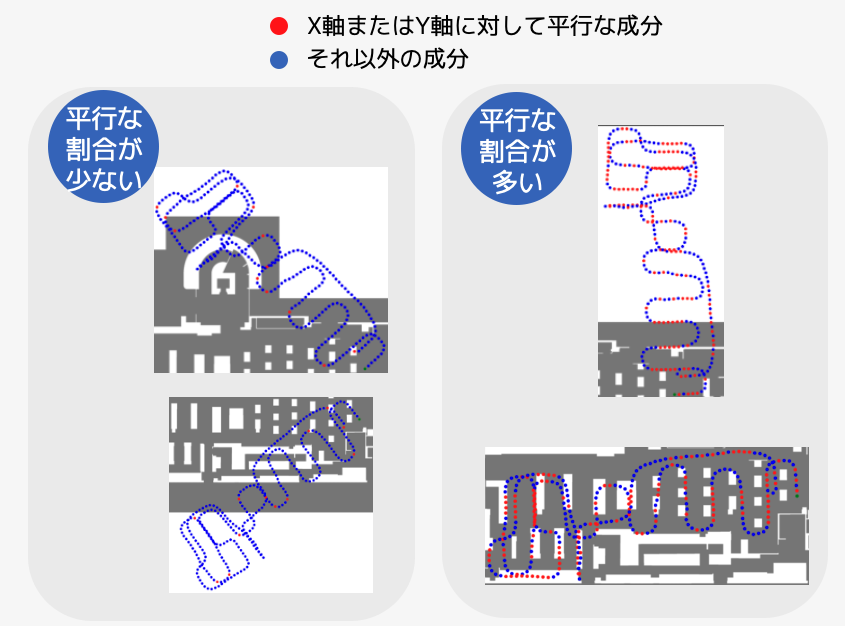
\includegraphics[width=\linewidth]{image/parallel.jpg}
	\caption{x軸とy軸に対して平行な成分の割合}    \label{fig:parallel}
\end{figure}

第二段階では,フロアマップ上の歩行可能領域の情報を活用する.
具体的には,各候補角度で軌跡を回転させ,その軌跡上の点がフロアマップ上で歩行可能な
領域に含まれる割合を計算する.

図\ref{fig:pdr-rotate}は,この補正処理を適用した結果を示している.
補正後の軌跡は建物の構造に整合し,正解軌跡により近い形状となっている.
この手法は,特に廊下や部屋が格子状に配置された一般的なオフィスビルなどの
環境で効果的である.

\begin{figure}[H]
	\centering
	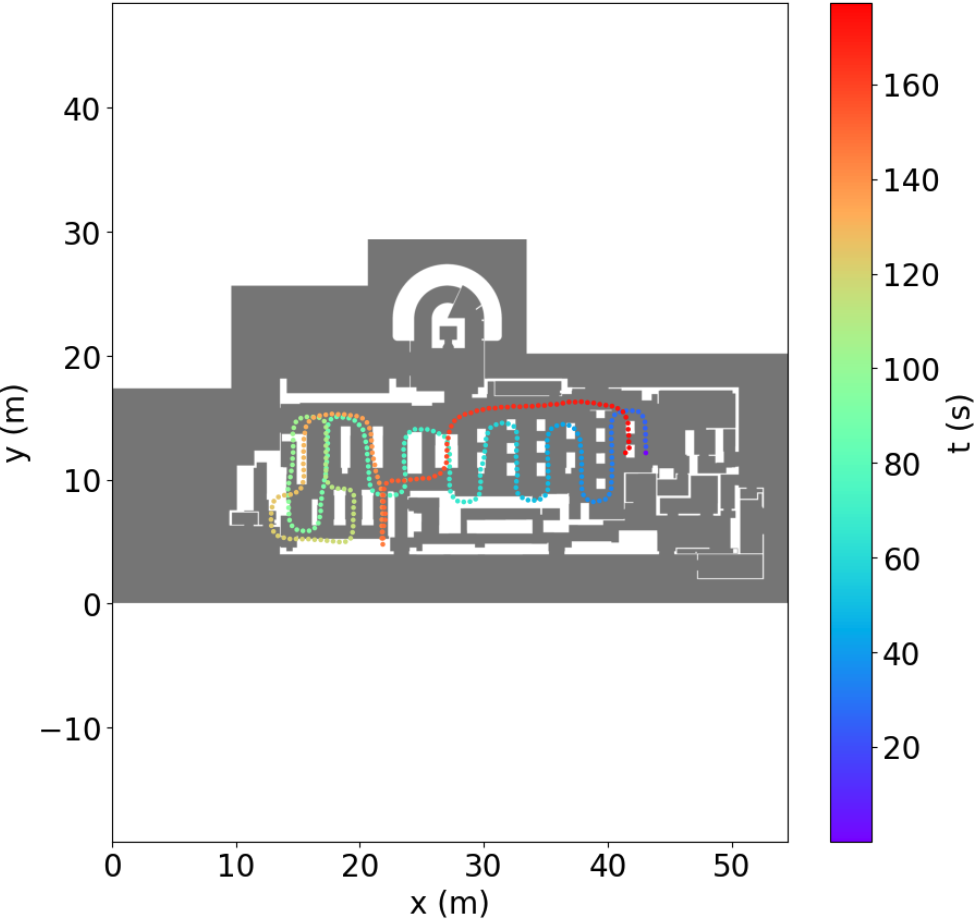
\includegraphics[width=\linewidth]{image/pdr-rotate.jpg}
	\caption{初期進行方向の補正後の軌跡}    \label{fig:pdr-rotate}
\end{figure}





% TODO: 3.段落が短すぎるのでまとめたり増やす必要がある.
\subsubsection{送信機の基地局情報を用いた初期進行方向の補正}

フロアマップ情報を用いた初期進行方向補正手法は,建物の構造に依存するため,オープンスペースが
多い環境などでは効果的に機能しない場合がある.このような環境でも適用可能な
手法として,本ライブラリでは無線送信機の基地局情報を活用した補正手法を
提供している.

この手法を利用するために必要な情報は主に2つある.1つ目は歩行者が
移動中に収集した信号スキャンデータである.これは歩行者の
スマートフォンが周辺の無線送信機を検知した際に記録される情報で,
各送信機のID,検知した時刻,そのときの電波強度(RSSI)が含まれている.
歩行者が送信機に近づいたり遠ざかると,この電波強度は
時間とともに変化する.2つ目は送信機の基地局情報である.
これは各送信機のIDとその送信機が実際に設置されている座標が
記録された情報である.

この手法はWirelessSignalCorrectorクラスとして実装されており,PDRによる推定位置と
これらの無線信号情報の関係性を利用する.図\ref{fig:ble-beacon-position}は,
xDR Challenge 2023環境におけるBLEビーコンの配置例を示している.各送信機は
既知の座標に固定されており,歩行者の移動に伴って受信されるRSSI値が変化する.
この手法の利用例をListing\ref{lst:ble-beacon-position}に示す

% TODO: 2.データが1つしかないように見える.複数個あるのを表現した方がいいと思う.
% TODO: 2.captionの名前は検討した方がいいかも
\begin{lstlisting}[caption={WirelessSignalCorrectorの使用例},label=lst:ble-beacon-position,float=h]
# 送信機の基地局情報
transmitter_positions = pd.read_csv('transmitter_positions.csv')
# transmitter_id: "f2:65:d1:87:a4:2c"
# x: 15.2  # メートル
# y: 24.8  # メートル
# floor: "floor_5"

# 歩行中に収集したスキャンデータ
signal_realtime_scans = pd.read_csv('signal_scans.csv')
# ts: 1234567890.123  # タイムスタンプ(秒)
# transmitter_id: "f2:65:d1:87:a4:2c"  # 送信機ID
# rssi: -68  # 電波強度(dBm)

# WirelessSignalCorrectorの初期化と補正の実行
wireless_corrector = WirelessSignalCorrector(
    signal_realtime_scans=signal_realtime_scans,
    transmitter_positions=transmitter_positions,
    rssi_threshold=-70  # 電波強度の閾値(dBm)
)
\end{lstlisting}

\begin{figure}[H]
    \centering
    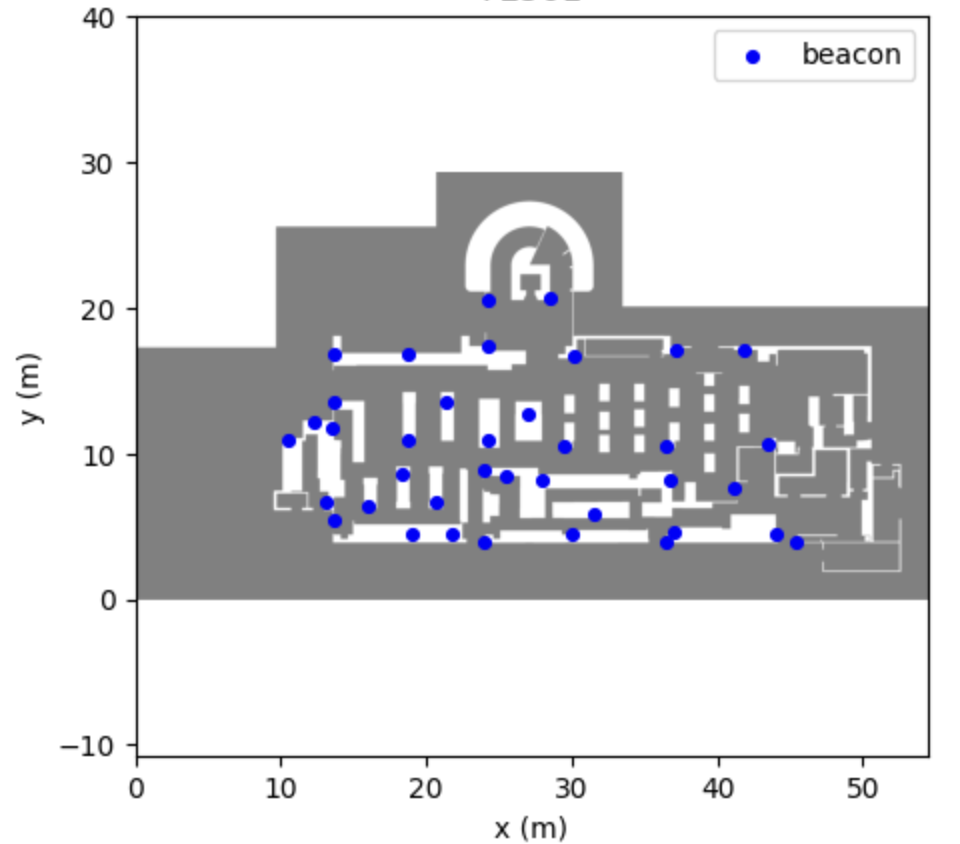
\includegraphics[width=\linewidth]{image/ble-beacon-position.jpg}
    \caption{送信機の配置例(xDR Challenge 2023環境)}    \label{fig:ble-beacon-position}
\end{figure}

% TODO: 2.RSSIの値はデータの上位何%という風に決めた方がいいかも.
% 多くのビーコンを使用してなんとなくの全体像を把握するの重要なポイントな気がする

まず受信した電波強度に対して閾値処理を行う.デフォルトではRSSIが-70dBmより
強い信号のみを使用する.この値は一般的な無線信号の減衰特性を考慮して
設定されており,およそ3メートル程度の範囲内での受信信号に相当する.
この閾値は環境やユースケースに応じて調整可能であり,WirelessSignalCorrectorの
初期化時にrssi\_thresholdパラメータとして指定できる.例えば
与えられる信号スキャンデータの電波強度が強い割合が小さい場合は-80dBm程度に緩和し,
逆に割合が多い場合は-65dBm程度に厳格化するといった調整が可能である.


この手法の特徴は建物の構造に依存せず,送信機が適切に配置されて
いれば任意の環境で適用可能な点にある.また電波強度の閾値の調整によって
補正の精度と信頼性のバランスを制御できる.ただしこの手法の
効果は送信機の配置密度や,環境内での電波伝搬特性に大きく
影響される点には注意が必要である.

次に選択された各信号について,受信時刻に最も近い推定軌跡上の
ポイントを特定する.図\ref{fig:ble-merge}は,この対応付けの結果を
可視化したものである.軌跡上のポイントは時間経過に応じて色付けされており,
青色のポイントは対応する送信機の位置を示している.

最後にこれらの対応点間の距離の総和が最小となるように軌跡全体の回転角度を
最適化する.受信時刻$t$における軌跡上の点と対応するビーコン基地局との
距離の総和$D(\theta)$を以下の式で表す:

\begin{equation}
D(\theta) = \sum_{t} \sqrt{(x_t(\theta) - b_x^t)^2 + (y_t(\theta) - b_y^t)^2}
\end{equation}

ここで$(x_t(\theta), y_t(\theta))$は角度$\theta$で回転させた軌跡上の
時刻$t$における座標,$(b_x^t, b_y^t)$は対応するBLEビーコン基地局の座標を表す.

\begin{equation}
\theta_{\mathrm{opt}} = \arg\min_{\theta \in [0, 2\pi]} D(\theta)
\end{equation}

% TODO: 2.このあたりの表現が微妙かも
この最適化問題は回転角度を$[0, 2\pi]$の範囲で探索することで解かれる.
この探索によりBLEビーコン基地局の位置と推定軌跡の位置関係が最も
整合する角度を見つけ最適な初期進行方向を決定できる.
% TODO: 2.グリードサーチしている文章の説明がない気がする

\begin{figure}[H]
	\centering
	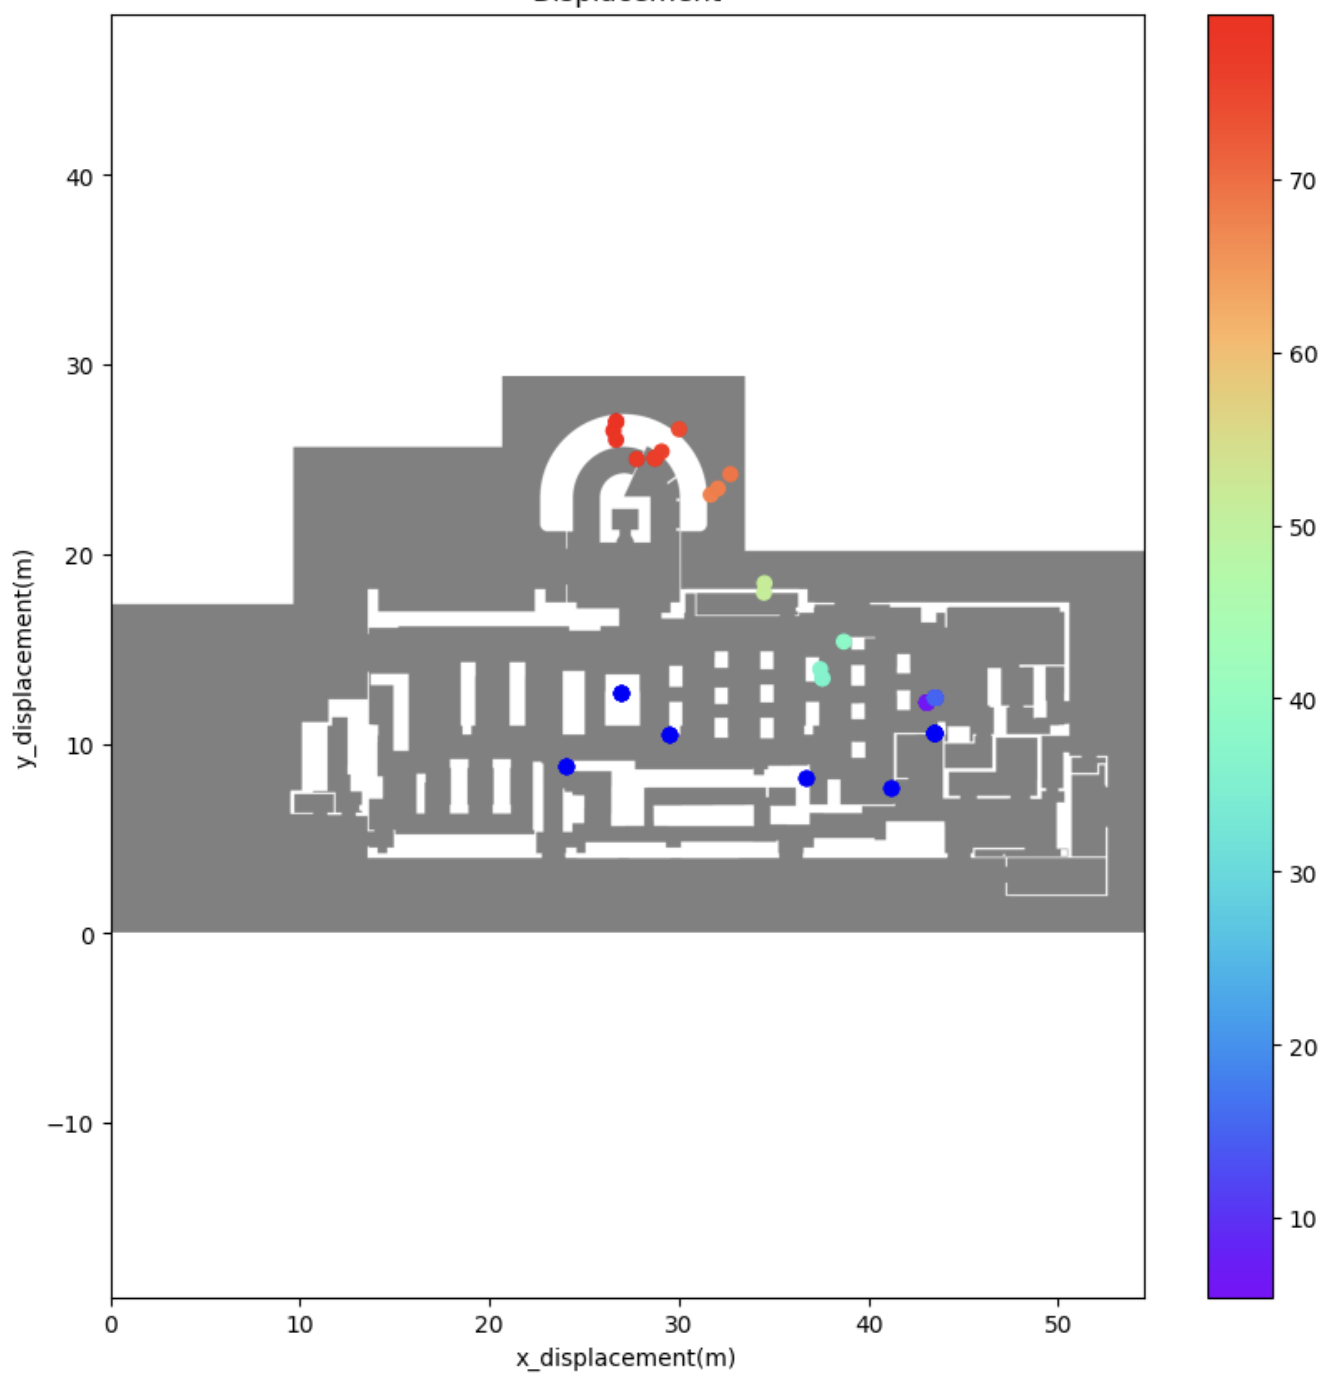
\includegraphics[width=\linewidth]{image/ble-merge.jpg}
	\caption{BLEビーコンの基地局の基地局情報}    \label{fig:ble-merge}
\end{figure}









\subsubsection{BLE フィンガープリントを用いた初期進行方向の補正}
% TODO:2. FPなのかフィンガープリントなのか統一した方がいいかも

BLEビーコンの基地局の位置情報を用いた補正手法は効果的である一方,基地局の
正確な位置情報を得るのが困難な場合がある.このような状況に対応するため,
本ライブラリではフィンガープリント(FP)を用いた補正手法も提供している.
この手法は,BLECorrectorクラスのFP機能として実装されている.

この手法を利用するために必要な情報は2つある.1つ目は前節と同様の
歩行者が移動中に収集したBLEビーコンのスキャンデータである.2つ目は
フィンガープリントデータである.これは事前に環境内の様々な位置で
計測された各ビーコンのID,電波強度,およびその計測位置の座標が
記録されたデータベースである.重要な点として,この手法では基地局の
正確な位置情報は必要としない.

この手法の利用例を以下に示す:


% TODO:3 BLECorrectorが被ってるのでキャプション名を変更した方がいいかも
\begin{lstlisting}[caption={BLECorrectorの使用例},label=lst:rotate-trajectory-using-ble-fingerprint,float=ht]
# フィンガープリントデータ
fingerprints = pd.read_csv('fingerprints.csv')
# ts: 1234567890.123  # 計測時刻(秒)
# x: 15.2            # 計測位置のx座標(メートル)
# y: 24.8            # 計測位置のy座標(メートル)
# bdaddress: "f2:65:d1:87:a4:2c"  # ビーコンID
# rssi: -68          # 電波強度(dBm)
# floor: "floor_5"   # フロア名

# BLECorrectorの初期化と補正の実行
corrector = BLECorrector(
    ble_realtime_scans=ble_scans,
    ble_fingerprints=fingerprints,
    rssi_threshold=-70
)
\end{lstlisting}


BLECorrectorのFPを用いた補正処理は,以下のように行われる.まず,
歩行者から受信した各BLE信号について,受信時刻$t$ごとに位置推定を行う.
各時刻において,受信したビーコンIDと同じデータポイントをFPデータベースから
抽出する.

各データポイントの重み$w$は,受信時刻$t$におけるRSSI値$r_t$と,
FPデータベース内の同じビーコンのRSSI値$r_f$との差に基づいて,
以下の式で計算される:

\begin{equation}
w_t = \exp\left(-\frac{(r_t - r_f)^2}{2\sigma^2}\right)
\end{equation}

ここで,$\sigma$は電波強度の標準偏差を表すパラメータであり,環境に応じて
調整可能である.この式はガウシアンカーネルに基づいており,RSSI値の差が
小さいほど大きな重みが与えられる.
% TODO:2.パスロスモデルの比重も増やせる説明をした方がいいかも

次に,これらの重みを用いて時刻$t$における推定位置$(p_x^t, p_y^t)$を
以下の式で計算する

\begin{equation}
p_x^t = \frac{\sum_{i=1}^{N_t} w_{t,i} x_i}{\sum_{i=1}^{N_t} w_{t,i}}, \quad
p_y^t = \frac{\sum_{i=1}^{N_t} w_{t,i} y_i}{\sum_{i=1}^{N_t} w_{t,i}}
\end{equation}

ここで,$(x_i, y_i)$はFPデータベース内の各データポイントの座標を表し,
$N_t$は時刻$t$において抽出されたデータポイントの総数である.この重み付き
平均により,その時刻のRSSI値と類似したデータポイントの座標がより強く
反映された推定位置が得られる.
% TODO:2.5 位置を推定した座標の図が欲しい
% TODO:2. 全体像を捉えて方向補正をするのが目的.なのでなんとなくこの辺にいそうというのが重要.
% 正確な位置を推定する必要はないといった方がいいかも

最適な回転角度の決定には,3.2.4節で導入した距離の総和$D(\theta)$を用いる.
ここでは,固定点として上記で推定された位置$(p_x^t, p_y^t)$を使用する.
最適な回転角度$\theta_{\mathrm{opt}}$は,前節と同様に距離の総和を
最小化する角度として決定される.

この手法の特徴は,基地局の正確な位置情報を必要としない点である.
その代わりに,事前に環境内で十分なFPデータを収集する必要があるが,
これは一度収集すれば継続的に使用できる.また,環境の変化に応じて
FPデータを更新することで,補正の精度を維持することができる.


TODO:2 この図を入れるなら何かしらの説明がいる.同じ初期進行方向補正だから図はいらない気がする
% \begin{figure}[H]
%     \centering
%     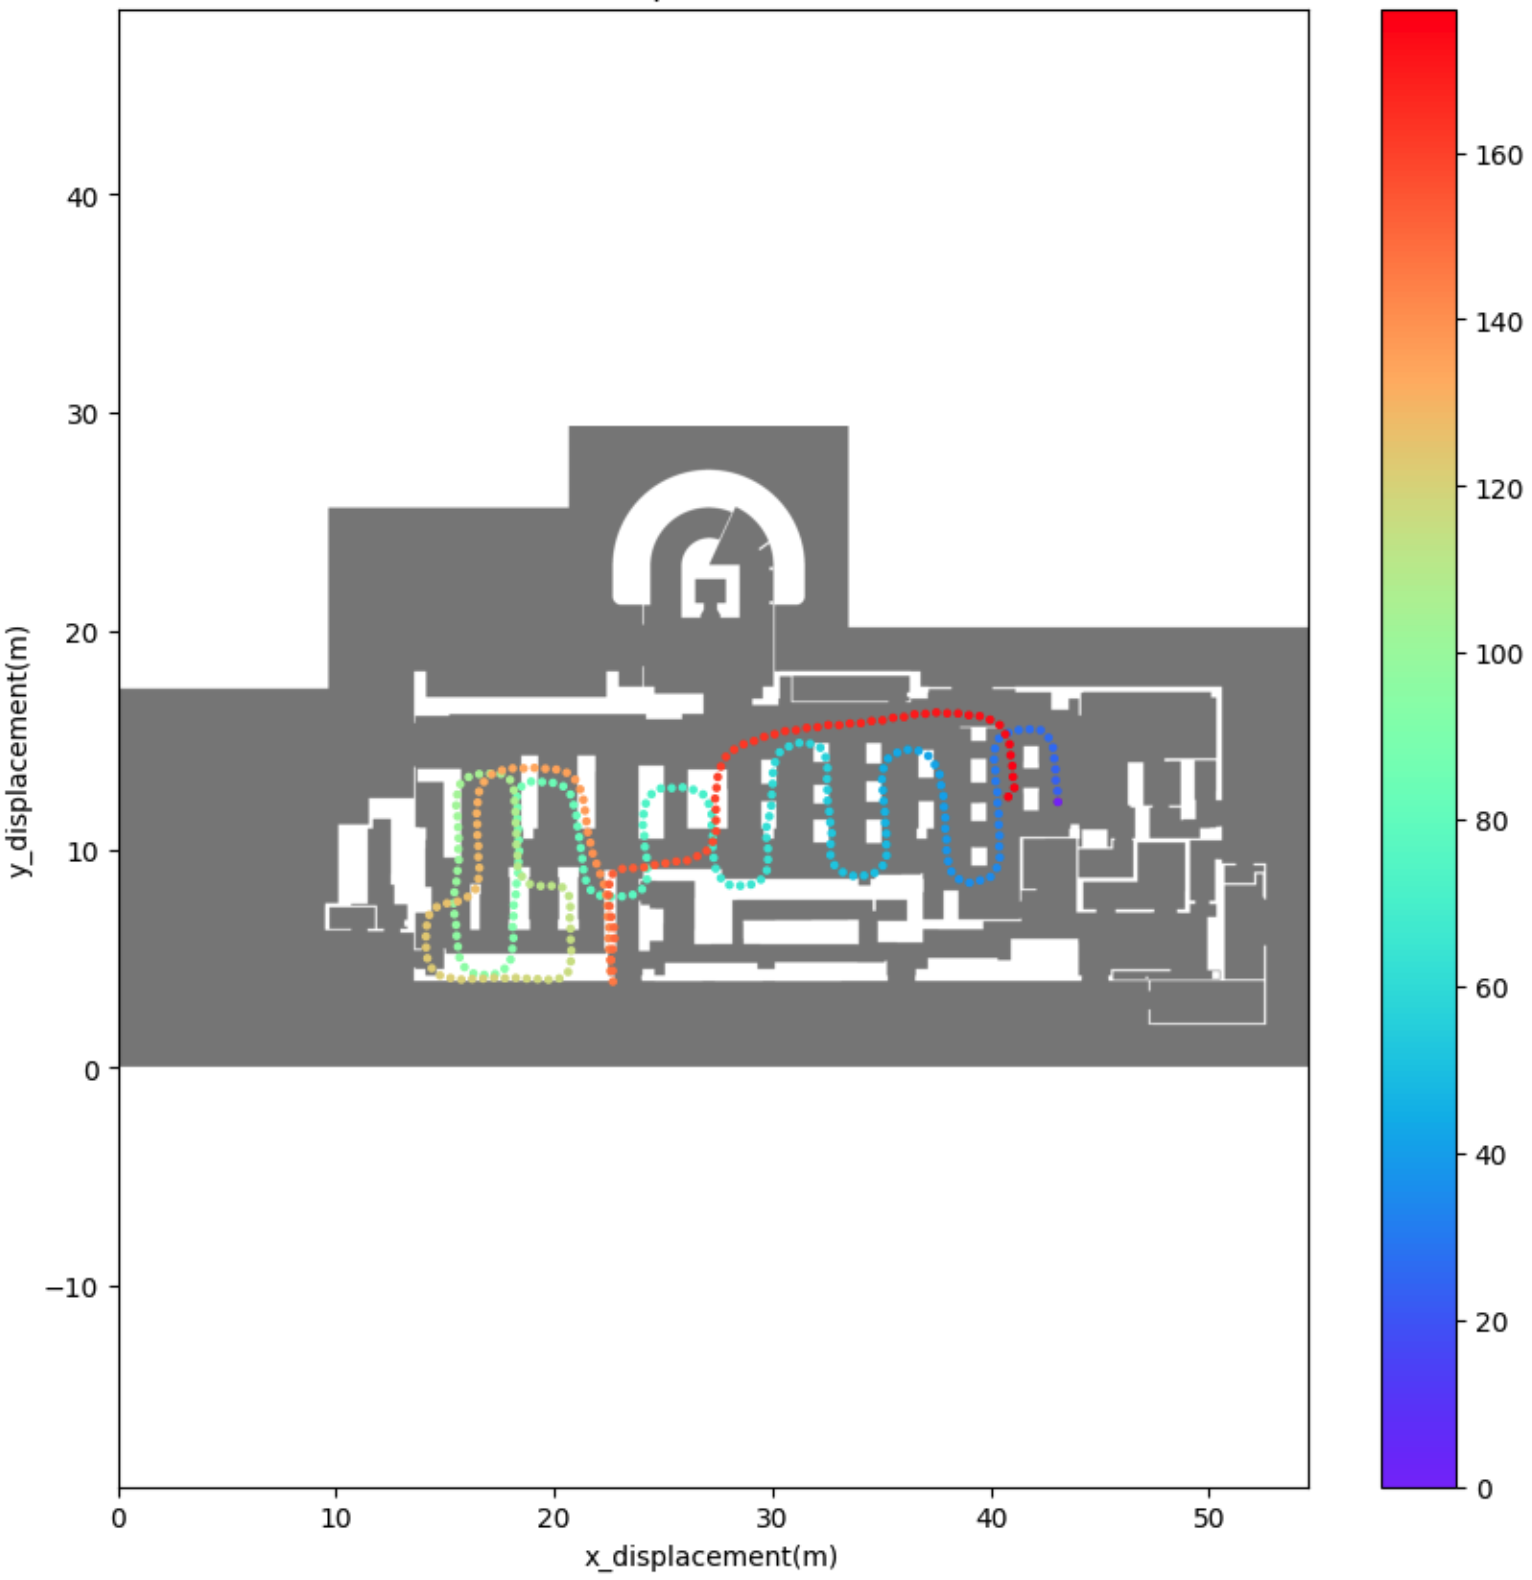
\includegraphics[width=\linewidth]{image/fingerprint-rotate.jpg}
%     \caption{BLEのFPを用いた補正後の軌跡}    \label{fig:fingerprint-rotate}
% \end{figure}

% TODO:2. 軌跡全体をみて最適化する形式だから十分なFPデータがなくても成り立つ



\subsubsection{フロアマップを用いた歩行可能座標への補正}
% TODO: 3.座標よりも座標の方がいいかもしれない

図\ref{fig:pdr-rotate}に示す軌跡には,人間が歩行不可能なを通過している
という重要な問題が残されている.

図\ref{fig:unwalkable_points}は歩行可能な座標を青色の点,
歩行不可能な座標を赤色の点を可視化したものである.
\begin{figure}[H]
    \centering
    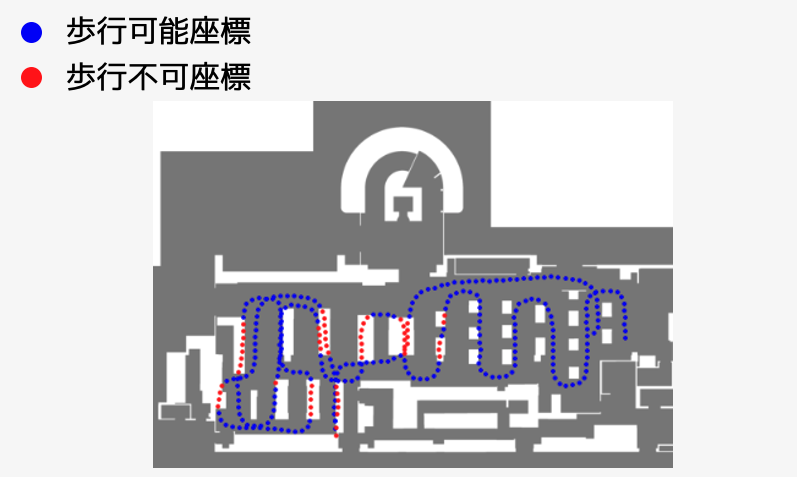
\includegraphics[width=\linewidth]{image/unwalkable_points.jpg}
    \caption{}    \label{fig:unwalkable_points}
\end{figure}


図\ref{fig:pdr-rotate}に示す軌跡には,人間が歩行可能座標ではない場所を
通過しているという重要な問題が残されている.図\ref{fig:walkable-points}は
ある軌跡上の点が歩行可能な座標であるか否かを示している.青色の点は
歩行可能な座標上に存在する点を,赤色の点は歩行可能ではない座標上に
存在する点を表している.この図から分かるように,軌跡の一部が壁や
障害物の存在する座標を通過している.このような軌跡は人間の実際の
歩行経路としては物理的に不適切である.この問題に対処するため,
本ライブラリではMapMatcherクラスの歩行可能座標補正機能を提供している.


この手法を利用するために必要な情報は,前節と同様のフロアマップ情報である.
このマップ情報を用いて,軌跡上の各点が歩行可能な座標に存在するように
補正を行う.

この手法の利用例を以下に示す:

\begin{lstlisting}
# MapMatcherの初期化
map_matcher = MapMatcher(
    pdr_estimator=estimator,  # PDREstimatorインスタンス
    floor_map=floor_map      # フロアマップ情報
)

# 歩行可能座標への補正
walkable_trajectory = map_matcher.correct_unwalkable_points(trajectory)
\end{lstlisting}

補正処理は以下の手順で行われる.まず,軌跡上の各点について,その座標が
フロアマップ上の歩行可能座標に存在するかを判定する.ある時刻$t$の
座標$(x_t, y_t)$が歩行不可能な座標に存在する場合,その点から最も近い

歩行可能な座標$(x_t^*, y_t^*)$を探索する.

この探索には幅優先探索(BFS)アルゴリズムを用いる.具体的には,現在の
座標から上下左右および斜め方向に探索を行い,最初に見つかった歩行可能な
座標を$(x_t^*, y_t^*)$として採用する.この際,探索はマップの境界を
超えないように制限される.

歩行可能な座標が見つかった場合,時刻$t$以降の全ての軌跡の座標を,
以下の式に従って平行移動する:

\begin{equation}
x_k' = x_k + (x_t^* - x_t), \quad y_k' = y_k + (y_t^* - y_t) \quad (k \geq t)
\end{equation}

ここで,$(x_k', y_k')$は補正後の座標,$(x_k, y_k)$は補正前の座標を表す.
この処理により,歩行不可能座標に存在していた点とそれ以降の軌跡が,
最も近い歩行可能な座標へと移動される.

この補正処理は軌跡の始点から順に適用される.図\ref{fig:map-matching}に
示すように,補正後の軌跡では全ての点が歩行可能な座標内に存在している.

なお,この補正処理は前節までの補正とは異なり,軌跡の進行方向は保持
したまま,位置のみを補正する特徴がある.

\begin{figure}[H]
    \centering
    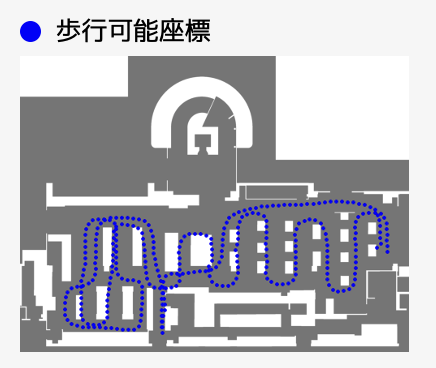
\includegraphics[width=\linewidth]{image/walkable-points.jpg}
    \caption{マップマッチング補正後の軌跡}    \label{fig:walkable-points}
\end{figure}


\section{気圧データを用いた3次元位置推定}



屋内環境における位置推定において,ユーザの3次元的な位置,特に現在いる階層の把握が必要となる.
PDRによる2次元軌跡推定では,ユーザの水平面上の移動は追跡できるものの,階層間の移動の検知は難しく,
特に複数階層を有する大規模な商業施設やオフィスビルでの屋内ナビゲーションにおいて大きな課題となる.

この課題に対し,これまでに様々なアプローチが提案されている.
Wi-Fiアクセスポイントの電波強度やBluetoothビーコンを利用する手法は既存のインフラを活用できる一方で,
電波強度が壁や人の移動の影響を受けやすく,各階での適切な配置が必要となる.
QRコードやARマーカーを用いる手法は高精度な階層識別が可能だが,
ユーザが意図的にマーカーをスキャンする必要があり,継続的な階層検知には適していない.
近年では,機械学習を用いて加速度センサやジャイロセンサのデータから階段の昇降を検知する手法も提案されている.
このアプローチは階段の昇降動作を高精度に検知できる一方で,エレベーターでの移動は検知できず,
また十分なデータセットによる訓練が必要となる.

本手法では気圧センサのデータを利用し,PDRによる2次元軌跡推定に垂直方向の移動検知を組み合わせた
3次元位置推定を行う.気圧センサは標準的なスマートフォンに搭載されており,
追加のインフラやハードウェアを必要としない.気圧は高度に応じて変化するため,
屋内環境においても階層の識別と移動検知が可能であり,
ユーザの明示的な操作を必要とせずエレベーターや階段での移動も追跡できる.

しかし,気圧データを用いた階層検知には,センサ自体のノイズや量子化誤差による変動,
気象条件による外気圧の変動,エレベーターや階段移動時の急激な気圧変化,
さらに建物内の空調システムによる局所的な気圧変化といった課題が存在する.
これらの課題に対処するため,本研究では安定区間検出とクラスタリングを組み合わせた
2段階の手法を提案する.以下,各段階について詳細に説明する.



\subsection{安定区間の検出}
気圧データから信頼性の高い階層情報を抽出するためには,まず安定した気圧値が観測される期間を特定する必要がある.
ここでの安定区間とは,一定時間以上にわたって気圧の変動が小さい期間を指す.
安定区間の検出では,気圧変動の閾値として0.02 hPa(約1.7mの高度差に相当)と,最小継続時間として4秒という
パラメータを用いる.

安定区間の検出では,指定された時間幅のウィンドウを用いて気圧データを走査する.
各ウィンドウ内での気圧の最大値と最小値の差が閾値以下である場合,そのウィンドウを安定区間として記録する.
この手法により,短期的なノイズの影響を受けにくい安定した気圧値を抽出することができる.

\begin{figure}[h]
	\centering
	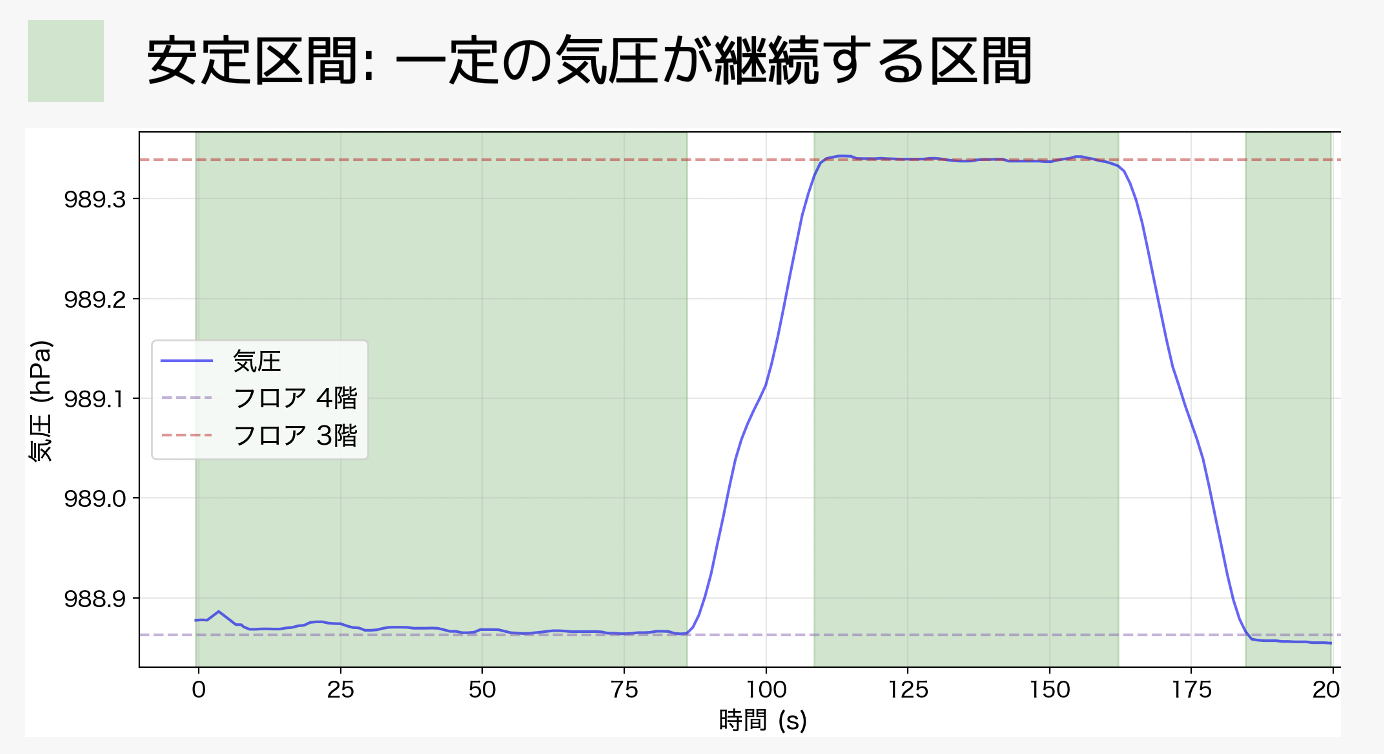
\includegraphics[width=\linewidth]{image/stable.jpg}
	\caption{安定歩行区間の検出}    \label{fig:stable_section}
\end{figure}

\subsection{DBSCANによる階層のグルーピング}
検出された安定区間内の気圧値に対して,DBSCANアルゴリズムを適用し階層のグルーピングを行う.
DBSCANは,クラスタ数を事前に指定する必要がなく建物の階数が未知の場合でも適用可能である.
また,ノイズの影響を受けにくく外れ値を自動的に除外できる特徴を持つ.
さらに,気圧値の分布が正規分布に従わない場合でも,任意の形状のクラスタを検出可能という利点がある.

DBSCANのパラメータは,建物の物理的特性に基づいて設定する.
具体的には,標準大気圧の高度による変化(約12 Pa/m)と標準的な階高(3.0 m)を考慮する.
クラスタ半径$\epsilon$は標準階高の半分の高度変化に相当する0.018 hPaとし,
最小サンプル数$minPts$は1と設定する.

クラスタリングにより得られた各グループの平均気圧値を計算し,これを階層の代表値として採用する.
その後,気圧値の大きさに基づいて階層番号を割り当てる.
具体的には,最も気圧値が大きい(最も低層の)クラスタから順に0から始まる整数値を割り当てる.
これにより,建物の物理的な構造と整合性のある階層番号付けが実現できる.

\subsection{階層間遷移の検知}
階層間の移動は,安定区間の間に観測される顕著な気圧変化として検出される.
本手法では,連続する安定区間の間の気圧の変化パターンを分析することで,
階層間の移動を検知する.

階層間の遷移検知において,まず時系列データ内で1.0秒以上の間隔が空いている箇所を特定し,
それを境界として異なる時間区間に分割する.次に,各時間区間について,
その区間内の気圧値に対応する軌跡データを抽出する.
最後に,抽出された軌跡データとDBSCANにより特定された階層の気圧範囲を照合することで,
各時間区間における階層を特定する.この手法により,エレベーターや階段による移動,
さらには一時的な滞在を含む複雑な移動パターンも適切に検出することが可能となる.

\subsection{適用例}
本手法を実データに適用した例を図\ref{fig:move_between_floor}に示す.
この例では,気圧データから複数の階層が識別され,
それぞれの階層における滞在時間と移動の様子が明確に可視化されている.
気圧データの分析から,各階層を代表する気圧値が物理的に妥当な間隔で分離されており,
階層間の移動が連続的な気圧変化として捉えられていることが確認できる.
また,各階層での滞在時における気圧値の安定性も明確に示されている.

特に注目すべき点として,安定区間の検出とDBSCANによるグルーピングを組み合わせることで,
センサノイズや一時的な気圧変動に影響されることなく,信頼性の高い階層識別が
実現できていることが挙げられる.この結果は,提案手法が実環境における
3次元位置推定に有効であることを示している.


\begin{figure}[h]
	\centering
	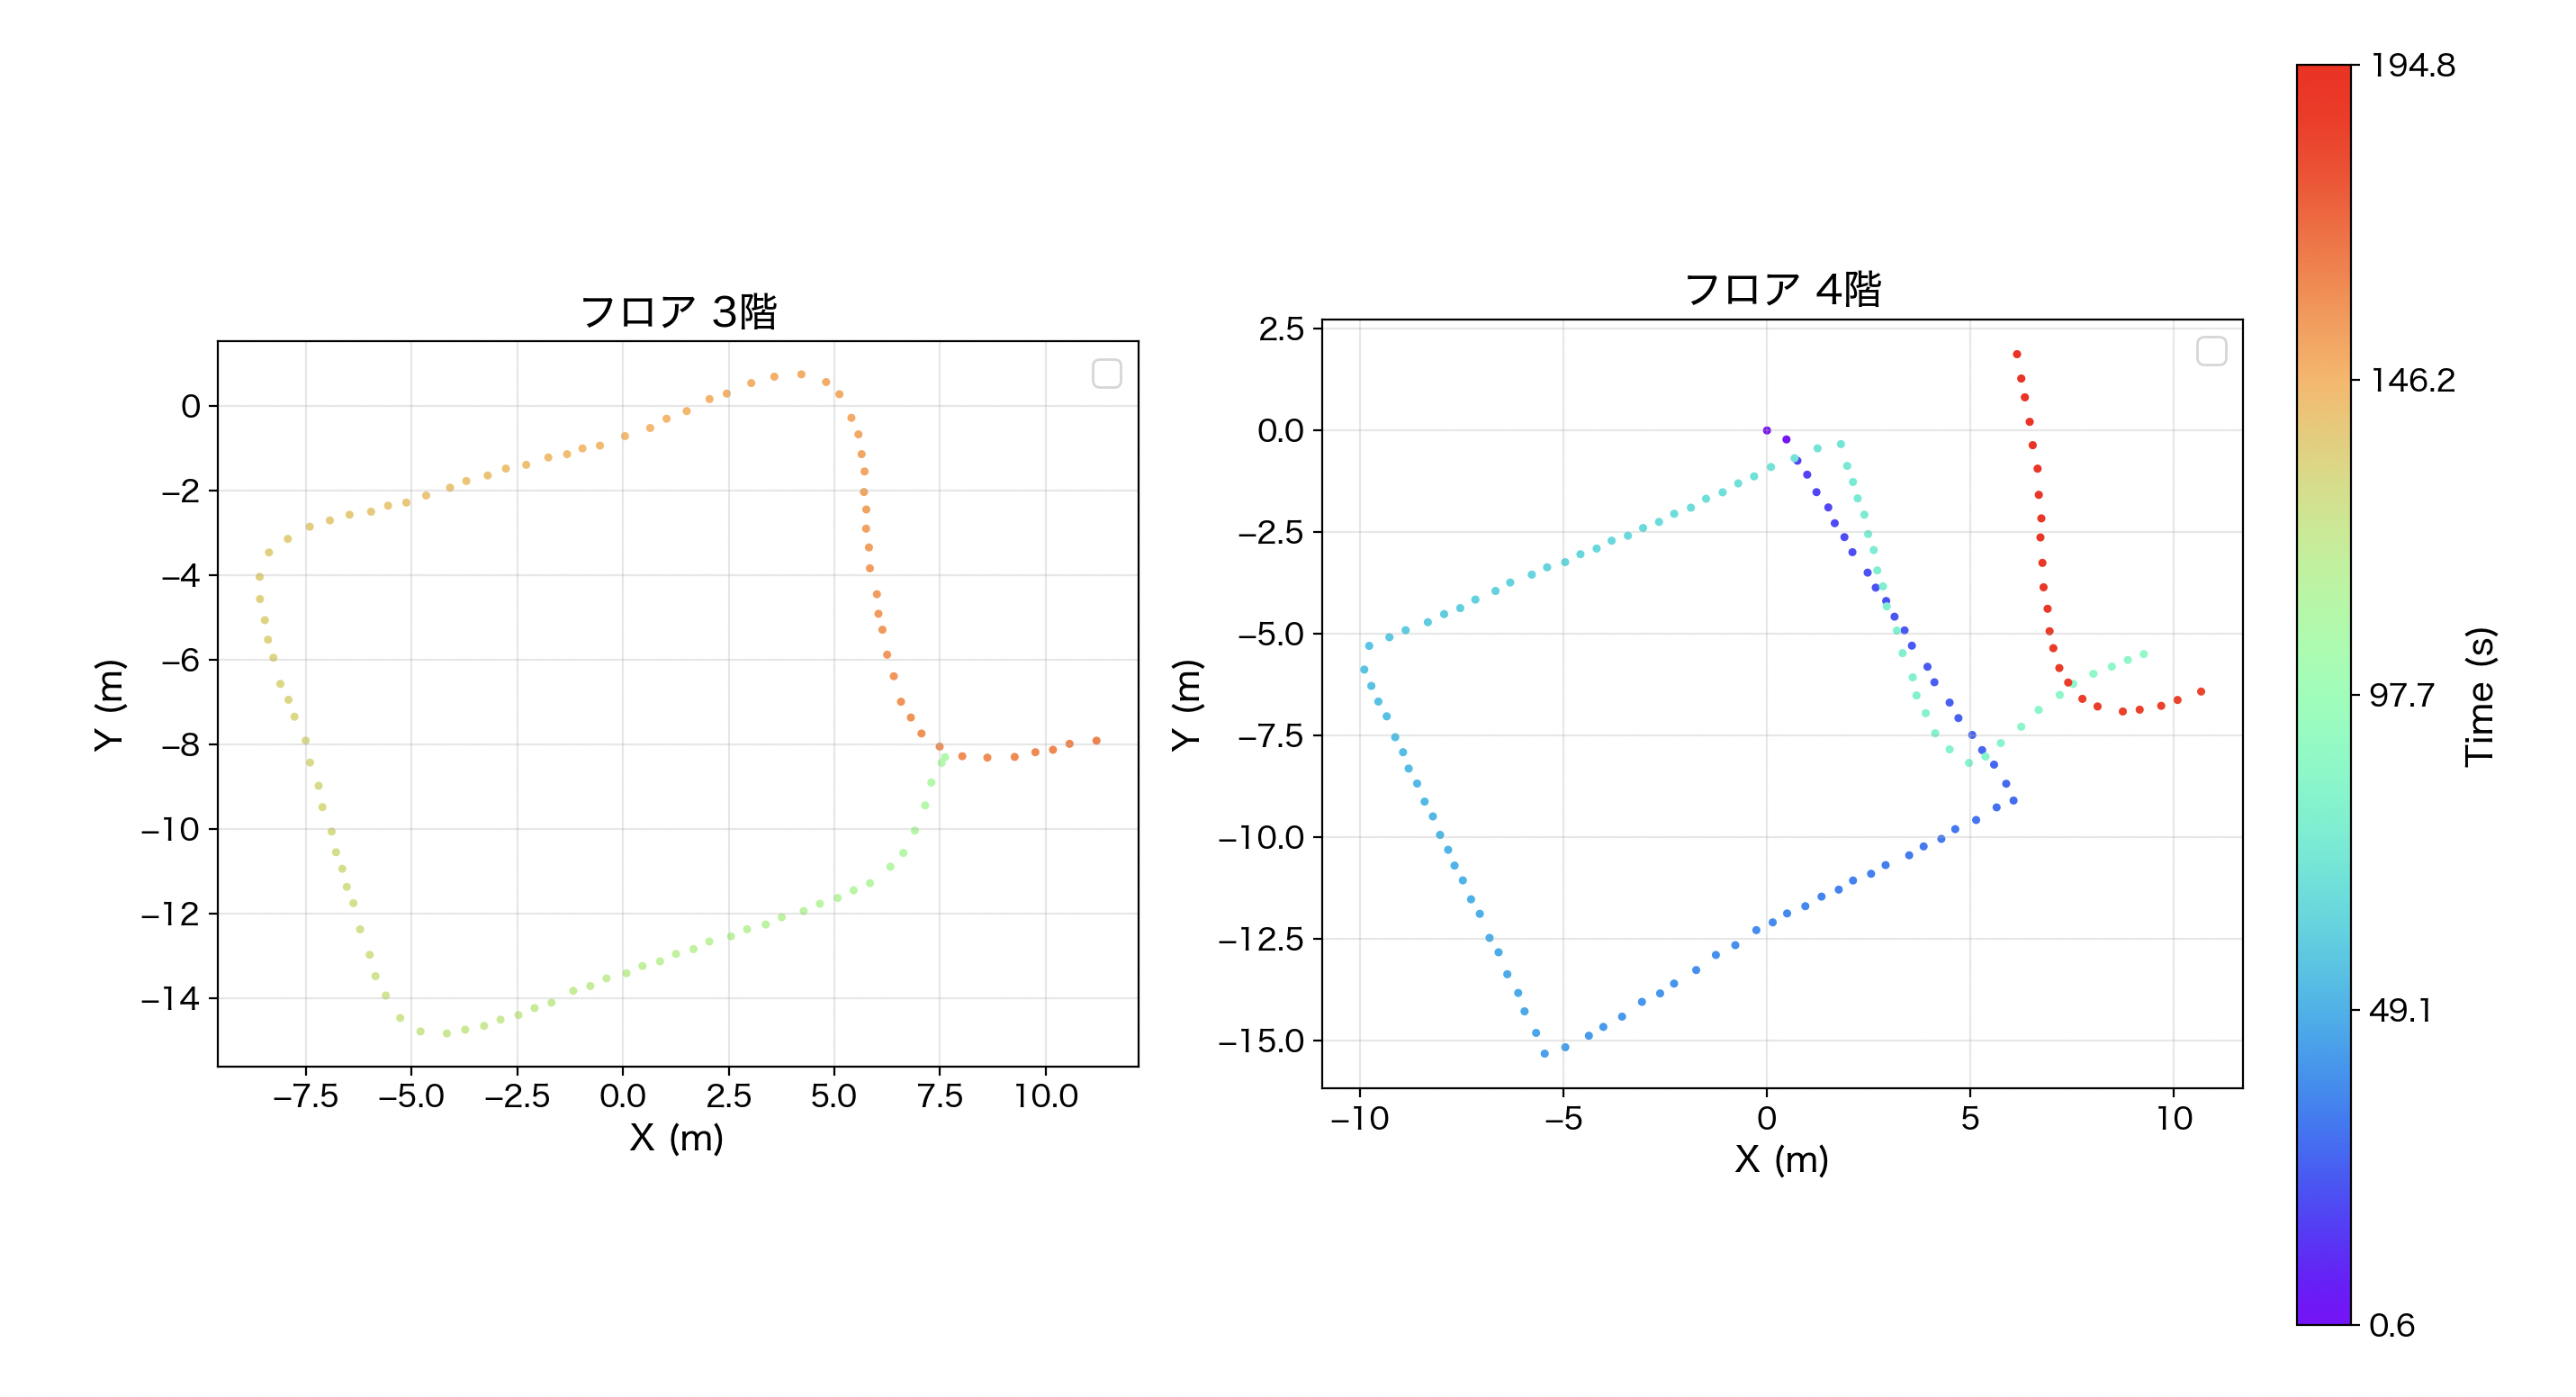
\includegraphics[width=\linewidth]{image/move_between_floor.jpg}
	\caption{適用例}    \label{fig:move_between_floor}
\end{figure}


